

\documentclass[]{book}

%These tell TeX which packages to use.
\usepackage[utf8]{inputenc}
\usepackage{array,epsfig}
\usepackage{amsmath}
\usepackage{amsfonts}
\usepackage{amssymb}
\usepackage{amsxtra}
\usepackage{amsthm}
\usepackage{mathrsfs}
\usepackage{color}
\usepackage{natbib}
\usepackage{graphicx}
\usepackage[english, russian]{babel}
\usepackage{mathtools}
\usepackage{rotating}
\usepackage{tikz}
\usepackage{wrapfig}
\usepackage{multicol}
\usepackage{enumitem}

%Here I define some theorem styles and shortcut commands for symbols I use often
\theoremstyle{definition}
\newtheorem{defn}{Определение}
\newtheorem{thm}{Теорема}
\newtheorem{cor}{Следствие}
\newtheorem*{rmk}{Замечание}
\newtheorem{lem}{Лемма}
\newtheorem*{joke}{Шутка}
\newtheorem{ex}{Пример}
\newtheorem*{soln}{Решение}
\newtheorem{prop}{Утверждение}

\newcommand{\lra}{\longrightarrow}
\newcommand{\ra}{\rightarrow}
\newcommand{\surj}{\twoheadrightarrow}
\newcommand{\graph}{\mathrm{graph}}
\newcommand{\bb}[1]{\mathbb{#1}}
\newcommand{\Z}{\bb{Z}}
\newcommand{\Q}{\bb{Q}}
\newcommand{\R}{\bb{R}}
%\newcommand{\C}{\bb{C}}
\newcommand{\N}{\bb{N}}
\newcommand{\M}{\mathbf{M}}
\newcommand{\m}{\mathbf{m}}
\newcommand{\MM}{\mathscr{M}}
\newcommand{\HH}{\mathscr{H}}
\newcommand{\Om}{\Omega}
\newcommand{\Ho}{\in\HH(\Om)}
\newcommand{\bd}{\partial}
\newcommand{\del}{\partial}
\newcommand{\bardel}{\overline\partial}
\newcommand{\textdf}[1]{\textbf{\textsf{#1}}\index{#1}}
\newcommand{\img}{\mathrm{img}}
\newcommand{\ip}[2]{\left\langle{#1},{#2}\right\rangle}
\newcommand{\inter}[1]{\mathrm{int}{#1}}
\newcommand{\exter}[1]{\mathrm{ext}{#1}}
\newcommand{\cl}[1]{\mathrm{cl}{#1}}
\newcommand{\ds}{\displaystyle}
\newcommand{\vol}{\mathrm{vol}}
\newcommand{\cnt}{\mathrm{ct}}
\newcommand{\osc}{\mathrm{osc}}
\newcommand{\LL}{\mathbf{L}}
\newcommand{\UU}{\mathbf{U}}
\newcommand{\support}{\mathrm{support}}
\newcommand{\AND}{\;\wedge\;}
\newcommand{\OR}{\;\vee\;}
\newcommand{\Oset}{\varnothing}
\newcommand{\st}{\ni}
\newcommand{\wh}{\widehat}
\newcommand{\ep}{\varepsilon}
\renewcommand{\leq}{\leqslant}
\newcommand{\tr}{\small{T}}

\DeclareMathOperator{\Ima}{Im}
\DeclareMathOperator{\Ker}{Ker}

%Pagination stuff.
\setlength{\topmargin}{-.3 in}
\setlength{\oddsidemargin}{0in}
\setlength{\evensidemargin}{0in}
\setlength{\textheight}{9.in}
\setlength{\textwidth}{6.5in}
\pagestyle{empty}

\everymath{\displaystyle}

\linespread{1.5}


\usepackage[labelformat=empty]{caption}


\begin{document}


\begin{center}
{\Large Задачи для подготовки к КР по геометрии}\\
\textbf{ВШЭ ЦПМ 1 курс КР 22 октября}\\ %You should put your name here
2018/19 учебный год %You should write the date here.
\end{center}

%\vspace{0.2 cm}

\subsection*{1. Алгоритм Евклида}

\begin{enumerate}

%1 done

\item Птицефабрика фасует яйца в коробки, рассчитанные либо на дюжину
яиц, либо на 25 яиц. Сможет ли птицефабрика отсчитать покупателю ровно 401
яйцо, используя только такие коробки? Предполагается, что в каждой коробке лежит
ровно столько яиц, на сколько она рассчитана

\textbf{Решение:}

По сути нам надо решить уравнение $25x + 12y = 401$ в натуральных числах. $(5, 23)$ - является решением данного уравнения $\Longrightarrow$ \text{сможет.}

\textbf{Ответ: } сможет

%2 done
\item Найдите все решения в целых числах диофантова уравнения

$$16x + 27y = 214$$
\textbf{Решение:}

$(10,2)$ - частное решение. $\Longrightarrow$
$
\begin{cases}
   16x + 27y = 214 \quad (1) \\
   16\cdot 10 + 27\cdot 2 = 214\ (2)
 \end{cases}\\
$
$(1) - (2): 16(x-10) + 27(y-2) = 0$\\
$16(x-10) = 27(2-y)$
$
\begin{cases}
   x = 10 + 27k \\
   y = 2 - 16k
\end{cases}
k\in\bb{Z}$ \\

\textbf{Ответ: } $(10+27k, 2-16k),\: k\in\bb{Z}$


%3 done
\item Найдите наибольший общий делитель многочленов $x^{30} - 1$ и $x^8 - 1$

\textbf{Решение:}

Многочлен $d(x)$ называется наибольшим общим делителем многочленов $f(x)$ и $g(x)$, если выполнены условия:

1)	$d(x)$ является делителем $f(x)$ и $g(x)$ (т. е. это общий делитель);

2)	если какой-либо $h(x)$ делит $f(x)$ и $g(x)$, то $h(x)$ делит и $d(x)$ (т. е. это наибольший общий делитель).

Поделим $x^{30} -1$ на $x^8 - 1$ с остатком:
$$x^{30} - 1 = (x^{22} + x^{14} + x^6)\cdot (x^8 - 1) + x^6 - 1$$
Получили остаток $x^6 - 1$

Теперь поделим $x^8 - 1$ на $x^6 - 1$ с остатком:
$$x^8 - 1 = x^2\cdot(x^6 - 1) + x^2 - 1$$
Получили остаток $x^2 - 1$.
Теперь поделим $x^6 - 1$ на $x^2 - 1$ с остатком:
$$x^6 - 1 = (x^4 + x^2 + 1)\cdot(x^2 - 1) + 0$$
Получили остаток 0, значит, последний ненулевой остаток есть НОД$(x^{30} - 1,\: x^8 - 1) = x^2 - 1$

\textbf{Ответ:} $x^2 - 1$.


%4 done
\item (Китайская теорема об остатках) Найдите все решения системы сравнений 
$$x \equiv 5 \pmod{8}, \quad x \equiv 2 \pmod{7}, \quad x \equiv 3 \pmod{15} $$
\textbf{Решение:}


$M = m_1\cdot m_2\cdot m_3 = 8\cdot 7\cdot 15 = 840$\\
$x_0 = M_1\cdot y_1\cdot C_1 + M_2\cdot y_2\cdot C_2 + M_3\cdot y_3\cdot C_3$ \\

1) $M_1 = \frac{M}{m_1} = \frac{840}{8} = 105$\\
$M_2 = \frac{M}{m_2} = \frac{840}{7} = 120$\\
$M_3 = \frac{M}{m_3} = \frac{840}{15} = 56$\\

2)$ C_1 = 5$\\
$C_2 = 2$\\
$C_3 = 3$\\

3)(1)$M_1\cdot y_1\equiv 1 \pmod {m_1}$\\
$105\cdot y_1\equiv 1 \pmod {8}$\\
$y_1\equiv 1 \pmod {8}$\\
(2)$M_2\cdot y_2\equiv 1 \pmod {m_2}$\\
$120\cdot y_2\equiv 1 \pmod {7}$\\
$y_2\equiv 1 \pmod {7}$\\
$M_3\cdot y_3\equiv 1 \pmod {m_3}$\\
$56\cdot y_3\equiv 1 \pmod {15}$\\
$y_3\equiv 11 \pmod {15}$\\

$x_0 = 105\cdot 1\cdot 5 + 120\cdot 1\cdot 2 + 56\cdot 11\cdot 3 = 2613$ \\
$x \equiv 2613 \pmod {840}$\\
$x \equiv 93 \pmod {840}$\\
\textbf{Ответ: } $x \equiv 93 \pmod {840}$


%5 done
\item Найдите натуральное число $x$, не превосходящее 120, такое что
$$x \equiv 1 \pmod{8}, \quad x \equiv 2 \pmod{5}, \quad x \equiv 0 \pmod{3} $$
\textbf{Решение:}

$M = m_1\cdot m_2\cdot m_3 = 8\cdot 5\cdot 3 = 120$\\
$x_0 = M_1\cdot y_1\cdot C_1 + M_2\cdot y_2\cdot C_2 + M_3\cdot y_3\cdot C_3$ \\

1) $M_1 = \frac{M}{m_1} = \frac{120}{8} = 15$\\
$M_2 = \frac{M}{m_2} = \frac{120}{5} = 24$\\
$M_3 = \frac{M}{m_3} = \frac{120}{3} = 40$\\

2)$ C_1 = 1$\\
$C_2 = 2$\\
$C_3 = 0 \Longrightarrow y_3$ \ \text{искать не надо, так как слагаемое } $M_3\cdot y_3\cdot C_3$ \text{будет равно} $0$\\

3)(1)$M_1\cdot y_1\equiv 1 \pmod {m_1}$\\
$15\cdot y_1\equiv 1 \pmod {8}$\\
$y_1\equiv 7 \pmod {8}$\\
(2)$M_2\cdot y_2\equiv 1 \pmod {m_2}$\\
$24\cdot y_2\equiv 1 \pmod {5}$\\
$y_2\equiv 4 \pmod {5}$\\

$x_0 = 15\cdot 7\cdot 1 + 24\cdot 4\cdot 2 + 40\cdot y_3\cdot 0 = 297$ \\
$x \equiv 297 \pmod {120}$\\
$x \equiv 57 \pmod {120}$\\
Так как x не превышает 120, то x = 57 — единственное решение.\\
\textbf{Ответ: } $57$




%6 done
\item Найдите квадратный многочлен $f$ с рациональными коэффициентами, такой что 
$$f(1) = 2, \quad f(2) = 20, \quad f(3) = 200$$

\textbf{Решение:}

$f(x) = ax^2+bx+c$\\
$
\begin{cases}
   a + b + c = 4\ (1)\\
   4a + 2b + c = 20\ (2) \\
   9a + 3b + c = 200\ (3)
 \end{cases}
$\\
 
$(2)-(1)\colon 3a + d = 16 \Longrightarrow b = 16 - 3a$\\
$(3)-(2)\colon 5a + b = 180 \Longrightarrow 5a + 16 - 3a = 180 \Longrightarrow 2a = 164 \Longrightarrow a = 82 \Longrightarrow b = -230$\\
$(1): 82 - 230 + с = 4 \Longrightarrow c = 152$\\
\textbf{Ответ: }$f(x) = 82x^2 - 230x + 152$

%7 done
\item Решите сравнение 
$$100x \equiv 999 \pmod{1001}$$
\textbf{Решение:}

$100x \equiv 999 \pmod{1001}$\\
$100x \equiv -2 \pmod{1001}$\\
$-10\cdot100x \equiv -10\cdot(-2) \pmod{1001}$ | (можно умножить на -10, т.к. оно взаимно просто с 1001)\\ 
$-1000x \equiv 20 \pmod{1001}$\\
$x \equiv 20 \pmod{1001}$\\
$x = 20 + 1001k,\: k \in \bb{Z}$.

\textbf{Ответ:} $ x = 20 + 1001k,\: k \in \bb{Z}$


%8 done
\item Решите уравнения в целых числах
$$ \text{а)}173x + 95y = 7; \text{б)}57x + 102y = 3;\ \text{в)}91x + 1001y = 6$$
\textbf{Решение:}
а)$173x + 95y = 7$\\
$(-6,11)$ - частное решение. $\Longrightarrow$
$
\begin{cases}
   173x + 95y = 7 \quad (1) \\
   173\cdot (-6) + 95\cdot 11 = 7\quad (2)
 \end{cases}\\
$

$(1) - (2)\colon 173(x+6) + 95(y-11) = 0$\\
$173(x+6) = 95(11-y)$
 
$
\begin{cases}
   x = -6 + 95k \\
   y = 11 - 173k
\end{cases}
k\in\bb{Z}$ \\

\textbf{Ответ: } $(-6+95k, 11-173k),\: k\in\bb{Z}$

б)$57x + 102y = 3$\\
$(9,-5)$ - частное решение. $\Longrightarrow$
$
\begin{cases}
   57x + 102y = 3 \quad (1) \\
   57\cdot 9 + 102\cdot (-5) = 3\quad (2)
 \end{cases}
$
\\

$(1) - (2): 57(x-9) + 102(y+5) = 0$\\
$57(x-9) = 102(-5-y)$
 
$
\begin{cases}
   x = 9 + 102k \\
   y = -5 - 57k
\end{cases}
k\in\bb{Z}$ \\

\textbf{Ответ: } $(9+102k, -5 - 57k),\: k\in\bb{Z}$

в)$91x + 1001y = 6$\\
$91x$ \vdots\ $13$ и $1001y$ \vdots\ $13 \Longrightarrow 6$\ \vdots\ $13$, \text{противоречие} $\Rightarrow \varnothing$\\
\textbf{Ответ: } $\varnothing$

%9 done
\item Решите уравнения в целых числах
$$ \text{а)}173x + 95y = 20000;\ \text{б)}57x + 102y = 10000$$
\textbf{Решение:}
а)$173x + 95y = 20000$\\
$(25,165)$ - частное решение. $\Longrightarrow$
$
\begin{cases}
   173x + 95y = 20000 \quad (1) \\
   173\cdot 25 + 95\cdot 165 = 3\quad (2)
 \end{cases}
$
\\

$(1) - (2): 173(x-25) + 95(y-165) = 0$\\
$57(x-25) = 102(165-y)$
 
$
\begin{cases}
   x = 24 + 95n \\
   y = 165 - 173n
\end{cases}
n\in\bb{N}$ \\
$y>0$ $\Longrightarrow$ $165 - 173n >0$ $\Longrightarrow$ $n = 0$ $\Longrightarrow$ $(25, 165)$ - единственное решение

\textbf{Ответ: } $(25, 165)$

б)$57x + 102y = 10000$\\
$57x$ \vdots\ $3$ и $102y$ \vdots\ $3 \Longrightarrow 10000$\ \vdots\ $3$, \text{противоречие} $\Rightarrow \varnothing$\\
\textbf{Ответ: } $\varnothing$

%10 done
\item Найдите многочлен $f(x)\in\bb{R}[x]$ степени не выше трёх, значения которого в точках $0, 1, 2 и 3$ совпадают со значениями функций.

$$\text{а)}2^x;\ \text{б)}\frac{1}{x+1};\text{в)}\sin{\frac{\pi x}{2}}$$

\textbf{Решение:}

$f(x) = ax^3+bx^2+cx+d$\\
а)$f(0) = 1$\\
$f(1) = 2$\\
$f(2) = 4$\\
$f(3) = 8$\\
1)$0+0+0+d=1$ $\Longrightarrow$ $d=1$\\
2)$a+b+c+1=2$ $\Longrightarrow$ $a+b+c=1$\\
3)$8a+4b+2c+1=4$ $\Longrightarrow$ $8a+4b+2c=3$\\
4)$27a+9b+3c+1=8$ $\Longrightarrow$ $27a+9b+3c=7$

Получаем систему: 
$
\begin{cases}
   a+b+c=1 \quad (1) \\
   8a+4b+2c=3\quad (2) \\
   27a+9b+3c=7\quad (3)
 \end{cases}
$\\
$(2)-(1)\colon 7a+3b+c=2 \Longrightarrow c = 2-7a-3b$\\
$(3)-(2)\colon 19a+5b+c=4 \Longrightarrow c = 4-19a-5b$\\
Получаем: $2-7a-3b=4-19a-5b \Longrightarrow 6a+b-1=0  \Longrightarrow b=1-6a \Longrightarrow\ c=2-7a-3+18a = 11a-1$\\
$(1): a+1-6a+11a-1=1 \Longrightarrow 6a = 1 \Longrightarrow a = \frac{1}{6} \Longrightarrow b = 0, c =\frac{5}{6}$\\
\textbf{Ответ: } $f(x) = \frac{1}{6}x^3+\frac{5}{6}x+1$

б)$f(0) = 1$\\
$f(1) = \frac{1}{2}$\\
$f(2) = \frac{1}{3}$\\
$f(3) = \frac{1}{4}$\\
1)$0+0+0+d=1$ $\Longrightarrow$ $d=1$\\
2)$a+b+c+1=\frac{1}{2}$ $\Longrightarrow$ $a+b+c=-\frac{1}{2}$\\
3)$8a+4b+2c+1=\frac{1}{3}$ $\Longrightarrow$ $8a+4b+2c=-\frac{2}{3}$\\
4)$27a+9b+3c+1=\frac{1}{4}$ $\Longrightarrow$ $27a+9b+3c=-\frac{3}{4}$

Получаем систему: 
$
\begin{cases}
   a+b+c=-\frac{1}{2} \quad (1) \\
   8a+4b+2c=-\frac{2}{3}\quad (2) \\
   27a+9b+3c=-\frac{3}{4}\quad (3)
 \end{cases}
$\\
$(2)-(1)\colon 7a+3b+c=-\frac{1}{6} \Longrightarrow c = -\frac{1}{6}-7a-3b$\\
$(3)-(2)\colon 19a+5b+c=-\frac{1}{12} \Longrightarrow c = -\frac{1}{12}-19a-5b$\\
Получаем: $-\frac{1}{6}-7a-3b=-\frac{1}{12}-19a-5b  \Longrightarrow 6a + b - \frac{1}{24} =0  \Longrightarrow b= \frac{1}{24}- 6a  \Longrightarrow $\\

$c= -\frac{1}{6}-7a-\frac{3}{24} +18a = 11a -\frac{7}{24}$

$(1): a + \frac{1}{24} -6a + 11a -\frac{7}{24} = -\frac{1}{2} \Longrightarrow a = -\frac{1}{24} \Longrightarrow b = \frac{7}{24}, c =-\frac{3}{4}$

\textbf{Ответ: } $f(x) = -\frac{1}{24}x^3+\frac{7}{24}x^2-\frac{3}{4}x+1$

в)$f(0) = 0$\\
$f(1) = 1$\\
$f(2) = 0$\\
$f(3) = -1$\\
1)$0+0+0+d=0$ $\Longrightarrow$ $d=0$\\
2)$a+b+c+0=1$ $\Longrightarrow$ $a+b+c=1$\\
3)$8a+4b+2c+0=0$ $\Longrightarrow$ $8a+4b+2c=0$\\
4)$27a+9b+3c+0=-1$ $\Longrightarrow$ $27a+9b+3c=-1$

Получаем систему: 
$
\begin{cases}
   a+b+c=1 \quad (1) \\
   8a+4b+2c=0\quad (2) \\
   27a+9b+3c=-1\quad (3)
 \end{cases}
$\\
$(2)-(1)\colon 7a+3b+c=-1 \Longrightarrow c = -1-7a-3b$\\
$(3)-(2)\colon 19a+5b+c=-1 \Longrightarrow c = -1-19a-5b$\\
Получаем: $-1-7a-3b=-1-19a-5b  \Longrightarrow 6a+b=0 \Longrightarrow b=6a \Longrightarrow c=-1-7a+18a = 11a-1$\\
$(1): a-6a+11a-1=1 \Longrightarrow 6a = 2 \Longrightarrow a = \frac{1}{3} \Longrightarrow b = -2, c =\frac{8}{3}$\\
\textbf{Ответ: } $f(x) = \frac{1}{3}x^3-2x^2+\frac{8}{3}x$

%11 done
\item Найдите такие многочлены $f$ и $g$ с рациональными коэффициентами, что
$$f(x)(x^3-2)+g(x)(2+x+x^2)=1,$$
\text{и при этом степень $f$ и $g$ не больше $2$.}\\
\textbf{Решение:}\\
$f(x) = ax^2 + bx+ c\\
g(x) = dx^2 + ex+ f\\
a,b,c,d,e,f \in \bb{Q}\\
f(x)(x^3-2)-g(x)(2+x+x^2)=1\\
ax^5-2ax^2+bx^4-2bx+cx^3-2c+2dx^2+dx^3+dx^4+2ex+2x^2+ex^3+fx^2+fx+2f=ax^5+(b+d)x^4+(c+d+e)x^3+(2d-2a+e+f)x^2+(2e-2b+f)x+(2f-2c)=1$

$ \Longrightarrow
\begin{cases}
   a=0  \\
   b+d=0\\
   c+d+e=0 \\
   2d-2a+e+f = 0\\
   2e-2b+f=0\\
   2f-2c = 1
 \end{cases}
\Longrightarrow 
\begin{cases}
   a=0  \\
   b=0,5\\
   c=0,5 \\
   d= -0,5\\
   e=0\\
   f= 1
 \end{cases}
$\\
Ответ: $f(x) = 0,5x + 0,5,\ \ g(x) = -0,5x^2 + 1$

%12 done
\item Найдите такие рациональные числа a, b и c, что
$$\frac{1}{2+\sqrt[3]{2}+\sqrt[3]{4}}= a+b\sqrt[3]{2}+\sqrt[3]{4} $$
\textbf{Решение:}

$(a+b\sqrt[3]{2}+c\sqrt[3]{4})(2+\sqrt[3]{2}+\sqrt[3]{4}) = 1$\\
\text{Пусть } $x = \sqrt[3]{2} \Longrightarrow x^2 = \sqrt[3]{4}, x^3 = 2, x^4 = 2\sqrt[3]{2} = 2x$\\
$(a+bx+cx^2)(2+x+x^2)=1$\\
$cx^4+(b+c)x^3+(2c+b+a)x^2+(2b+a)x+2a=1$\\
$2xc+(b+c)\cdot 2+(2c+b+a)x^2+(2b+a)x+2a=1$\\
$(2c+b+a)x^2+(2b+2c+a)x+(2a+2b+2c)=1+0\cdot x+ 0\cdot x^2$\\
Получаем систему: 
$
\begin{cases}
   a+b+2c=0 \quad (1) \\
   2b+a+2c=0\quad (2) \\
   2a+2b+2c=1\quad (3)
 \end{cases}
$\\
$(2)-(1)\colon b=0$\\
$(3)-(1)\colon a=1$\\
$(1)\colon 1+0+2c=0 \Longrightarrow 2c = -1 \Longrightarrow c = -\frac{1}{2}$\\
\textbf{Ответ: } $(1, 0, -\frac{1}{2})$





\end{enumerate}

\subsection*{2. Евклидовы пространства}

\begin{enumerate}[resume]


%13 done
\item Докажите, что площадь $|\omega(u, v)|$ параллелограмма, натянутого на векторы u и v можно считать по формуле:
$$\text{a) \ } |\omega (u, v)| = \sqrt{det \begin{pmatrix}
(u, u)  &  (u,v) \\
(v, u)  &  (v, v)\\
\end{pmatrix}} $$
$$\text{б) \ } |\omega (u, v)| = |u||v||\sin{\varphi}| $$
\textbf{Решение:}\\
а) Пусть $e_1, e_2$ - ортогональный базис в плоскости $<u, v>$. \\
$u = ae_1 + be_2$, $v = ce_1 + de_2$ => $\omega(u, v) = ad - bc = (u, e_1)(v, e_2) - (u, e_2)(v, e_1) = x_1y_2 - x_2y_1$ (заменили $(u, e_1) = a = x_1, (u, e_2) = b = x_2, (v, e_1) = c = y_1, (v, e_2) = d = y_2$).\\
$(u, u) = (u, e_1)^2 + (u, e_2)^2 = x_{1}^2 + x_{2}^2$\\
$(v, v) = y_{1}^2 + y_{2}^2$\\
$(u, v) = (v, u) = (u, e_1)(v, e_1) + 0 + 0 + (u, e_2)(v, e_1) = x_1y_1 + x_2y_2$\\
$$|\omega (u, v)| = \sqrt{det \begin{pmatrix}
(u, u)  &  (u,v) \\
(v, u)  &  (v, v)\\
\end{pmatrix}}  = \sqrt{(u,u)(v,v) - (u,v)(v,u)} = \sqrt{(x_{1}^2 + x_{2}^2)(y_{1}^2 + y_{2}^2) - (x_1y_1 + x_2y_2)^2} = x_1y_2 - x_2y_1$$ \\
б) $\cos{\varphi} = \frac{(u, v)}{|u|\cdot |v|}$\\
$$|\omega (u, v)| = \sqrt{det \begin{pmatrix}
(u, u)  &  (u,v) \\
(v, u)  &  (v, v)\\
\end{pmatrix}}  = \sqrt{(u, u)(v, v) - (\cos{\varphi} \sqrt{(u, u)} \sqrt{(v, v)})^2} = \sqrt{(u, u)(v, v)(\sin{\varphi})^2} = |u| |v| |\sin{\varphi}|.$$






%14 
\item Докажите неравенство Коши-Буняковского-Шварца в $\bb{R}^{n}: |(u,v)| \leq|u|\cdot|v|$\\
\textbf{Решение:}


%15
\item Найдите ортогональный базис в подпространстве:\\
a) заданном уравнением $ x_1 + x_2+ ... + x_n =0$\\
б) порожденный векторами (1,2,2,-1), (1,1,-5,3), (3,2,8,-7)\\
в) в ортогональном дополнении к предыдущему подпространству.\\
\textbf{Решение:}

%16 
\item Рассмотрим стандартное скалярное произведение на $\bb{R}^{n}$ и ограничим его на гиперплоскость $U = \{x_1+...+x_n = 0\}$. Через $e_1,..., e_n$ обозначим стандартный базис в  $\bb{R}^{n}$.\\
а)Найдите матрицу Грама скалярного произведения на $U$ в базисе ${\alpha}_{1}= e_1-e_2, ...,{\alpha}_{n}= e_{n-1}-e_{n} $\\
б)Найдите ортонормальный базис в U, применив ортогонализацию Грама-Шмидта к базису ${\alpha}_{1},...,{\alpha}_{n}$\\
\textbf{Решение:}



%17 done
\item Пусть $\Pi \subset \bb{R}^4$ - гиперплоскость, натянутая на векторы $(1,2,3,1), (1,2,3,2), (1,1,1,1)$.

(а) Найдите вектор единичной длины, перпендикулярный гиперплоскости $\Pi$

\textbf{Решение:}
$\begin{pmatrix}
1  &  2  &  3  &  1 \\
1  &  2  &  3  &  2 \\
1  &  1  &  1  &  1 \\
\end{pmatrix} \Rightarrow \begin{pmatrix}
1  &  0  &  1  &  0 \\
0  &  1  &  2  &  0 \\
0  &  0  &  0  &  0 \\
\end{pmatrix} \Rightarrow $ Перпендикулярный верктор будет (1, -2, 1, 0) $\Rightarrow$ единичный перпендикулрный ветор будет ($\frac{1}{\sqrt{6}}, {-}\frac{2}{\sqrt{6}}, \frac{1}{\sqrt{6}}, 0$)

(б) Найдите расстояние от точки $(6,3,6,5) \in \bb{R}^4$ до гиперплоскости $\Pi$\\
\textbf{Решение:}\\
Пусть все вектора выходят из начала координат.
Тогда общее уравнение плоскости: Ax+By+Cz+Dw=0\\
Получаем систему: 
$
\begin{cases}
   A+2B+3C+D=0 \quad (1) \\
   A+2B+3C+2D=0\quad (2) \\
   A+B+C+D=0\quad (3)
 \end{cases}
$\\
$(2)-(1)\colon D=0$\\
$(2)-(3)\colon B=-2C$\\
$(3)\colon A-2C+C=0 \Longrightarrow A = C$\\
$\Longrightarrow$ Уравнение плоскости: $Cx-2Cy+Cz=0|:C\\
x-2y+z=0$\\
$\rho = \frac{|Ax_0+By_0+Cz_0+Dw_o+E|}{\sqrt{A^2+B^2+C^2+D^2}}=\frac{|x_0-2y_0+z_0|}{\sqrt{1+4+1}}=\frac{|6-6+6|}{\sqrt{6}}=\sqrt{6}$\\
(в) Найдите длину ортогональной проекции вектора $(6,3,6,5)$ на гиперплоскость $\Pi$.\\
\textbf{Решение:}\\
 \begin{figure}[h!]
\centering
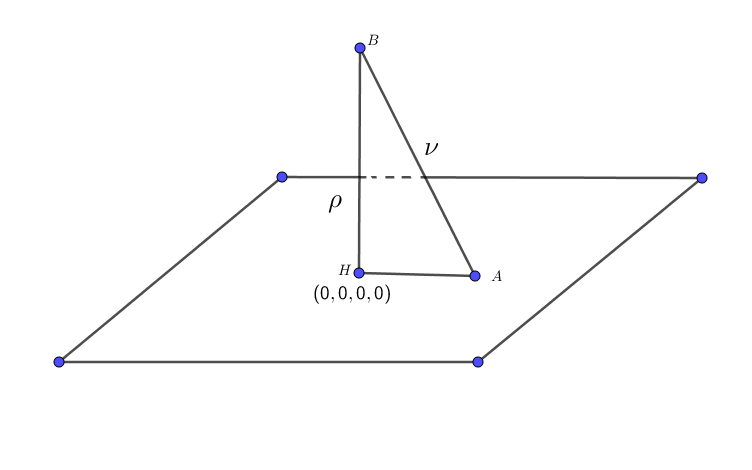
\includegraphics[scale=0.35]{17.PNG}
\end{figure}
$AH = \sqrt{v^2-\rho^2}, B(6,3,6,5)$\\
$|v^2|=\sqrt{36+9+36+25} = \sqrt{106}$\\
$AH = \sqrt{106-6}=10$\\

%18 
\item Найдите расстояние от точки p = (2,1,-3,4) до плоскости $\Pi =(2x_1 - 4x_2 - 8x_3 +13x_4 +19=0, x_1 +x_2 -x_3 + 2x_4 -1=0)$\\
\textbf{Решение:}\\


%19 
\item Найдите косинус угла между вектором $(1,2,3,4)$ и подпространством $\{x_1+x_2+x_3+x_4=1\}$\\
\textbf{Решение:}\\


%20 
\item Найдите расстояние между плоскостями $\Pi_1=(x_1 + x_3 +x_4 - 2x_5 -2=0, x_2 +x_3 -x_4 -x_5 -3=0, x_1 -x_2 +2x_3 -x_5 -3=0); \Pi_2=(1,-2,5,8,2)+ (0,1,2,1,2),(2,1,2,-1,1) $\\
\textbf{Решение:}\\

%21 done
\item Одинаковые шары в $\bb{R}^4$ расположены так, что их центры являются вершинами 4-мерного куба, причем сторона куба равна диаметру шара. Докажите, что между этими шарами можно разместить еще один шар того же размера, так что он будет касаться всех остальных шаров.

\textbf{Решение:}
Если мы хотим вписать шар, то как нетрудно заметить между противоположными вершинами куба должно быть расстояние $2x$ (диаметр шара $+$ два радиуса). Условия касания всех шаров с вписанным). Докажем, что расстояние равно $2x$. Поместим 1 вершину в координаты (0,0,0,0). Значит у противоположной вершины будут координаты $(x,x,x,x)$. Найдем расстояние: $\sqrt{x^{2} + x^{2} + x^{2} + x^{2}}=\sqrt{4x^{2}}=2{x}$.

Ч.Т.Д.



%22
\item Докажите что поворот R в $\bb{R}^{3}$ на угол $\varphi$ (против часовой стрелки) относительно оси, порожденной единичным вектором $e$, задается формулой:
$$R(u)=(1-\cos{\varphi})(v,e)e+\cos{\varphi}\ v+\sin{\varphi}[e,u]$$
\textbf{Решение:}

%23 
\item Найдите матррицу поворота в $\bb{R}^{3}$:\\
(a) на угол $\frac{2\pi}{3}$ относительно прямой $\{x_1=x_2=x_3\}$;\\
(б) на угол $\varphi$ относительно прямой $\{x_1=x_2=x_3\}$;\\
(в) на угол $\varphi$ относительно прямой $\{x_1=px_2=qx_3\}$, где $p, q\neq 0$\\
\textbf{Решение:}

%24 
\item Пусть $A$ - матрица линейного оператора из $\bb{R}^{3}$ в себя в стандартном базисе. Известно, что $AA^{t} = I$ (через $I$ обозначает единичная матрица),  и $det(A) =1$. Покажите, что оператор является повротом евклидова пространства $\bb{R}^{3}$ (относительно стандратного скалярного произведения).\\
\textbf{Решение:}

\end{enumerate}

\subsection*{3. Арифметика}

\begin{enumerate}[resume]

%25 done
\item (а) Докажите, что число вида $4k+3$  не представляется в виде суммы двух полных квадратов ни для какого натурального k.

\textbf{Решение:}
$4k+3 \equiv 3 \pmod{4}$, а квадраты по модулю 4 могут давать остатки 0, 1 $\Rightarrow$ сумма квадратов может дать 0, 1 или 2. ЧТД



(б) Докажите, что если целые m и n представляются в виде суммы двух полных квадратов, то их произведение mn тоже представляется в виде суммы двух квадратов.

\text{Решение:}

$m=(a^2 + b^2), n=(c^2 + d^2) m\cdot{n}=(a^2\cdot{c^2} + a^2\cdot{d^2}+b^2\cdot{c^2}+b^2\cdot{d^2})+2abcd - 2abcd = (ac+bd)^2 + (ad-bc)^2$ или $(ac-bd)^2 + (ad+bc)^2$



%26 done
\item Для каких остатков a по модулю p сравнение 
$$x^2 \equiv a \pmod{p}$$
разрешимо в целых числах, если p равно:\\
$(a)5$;\ \ $(\text{б})13$;\ \ $(\text{в})23$?\\
\text{Решение:}
(а)
\begin{minipage}{0.3\textwidth}

\begin{tabular}{ | l || l | l | l | l | l | }
\hline
$x$ & 0 & 1 & 2 & 3 & 4\\ \hline
$x^2$ & 0 & 1 & 4 & 4 & 1       \\  \hline

\hline
\end{tabular}
\end{minipage}
\\
(б)
\begin{minipage}{0.3\textwidth}

\begin{tabular}{ | l || l | l | l | l | l | l | l | l | l | l | l | l | l | }
\hline
$x$ & 0 & 1 & 2 & 3 & 4 & 5 & 6 & 7 & 8 & 9 & 10 & 11 & 12\\ \hline
$x^2$ & 0 & 1 & 4 & 9 & 3 & 12 & 10 & 10 & 12 & 3 & 9 & 4 & 1       \\  \hline

\hline
\end{tabular}
\end{minipage}
\\
(в)\\
\begin{minipage}{0.2\textwidth}

\begin{tabular}{ | l || l | l | l | l | l | l | l | l | l | l | l | l | l | l | l | l | l | l | l | l | l | l | l | }
\hline
$x$ & 0 & 1 & 2 & 3 & 4 & 5 & 6 & 7 & 8 & 9 & 10 & 11 & 12 & 13 & 14 & 15 & 16 & 17 & 18 & 19 & 20 & 21 & 22\\ \hline
$x^2$ & 0 & 1 & 4 & 9 & 16 & 2 & 12 & 3 & 18 & 12 & 8 & 6 & 6 & 8 & 12 & 18 & 3 & 12 & 2 & 16 & 9 & 4 & 1       \\  \hline

\hline
\end{tabular}
\end{minipage}

%27 done
\item Докажите, что если $p$ - нечетное простое число, то сравнение 
$x^{2} \equiv {a} \pmod{p}$ 
 
разрешимо в целых числах ровно для половины всех ненулевых остатков по модулю $p$.
\\
\textbf{Решение:}
\\ допустим, 
$a^{2} \equiv b^{2} \pmod{p}$ \\
тогда
$ (a-b)(a+b) \equiv {0} \pmod{p}$ \\
$=>$\\
$ (a-b) \equiv {0} \pmod{p}$ 
или
$ (a+b) \equiv {0} \pmod{p}$ \\
Значит, такой же остаток как и $a$ дает только остаток $p-a$.



%28
\item Докажите, что сравнение 
$$x^2+y^2+z^2\equiv 0\pmod{p}$$
имеет нетривиальное решение в целых числах(тривиальное решение - это решение $x\equiv y\equiv z\equiv 0 \pmod{p}$\\
\textbf{Решение:}
\textbf{!!!АХТУНГ!!!!Доказательство затычка!!!!!АХТУНГ!!!!}\\
Если кто знает как доказать без использования теоремы Лежандра о трех квадратах(Legendre's three-square theorem, на русском упоминаний не много, иногда ее доказательство у нас приписывают Гаусу) пишите не стесняйтесь(равно как изнания тривального доказательства этой теоремы)\\\\
По теореме Лежандра о трех квадратах, любое число представимо ввиде суммы трех квадратов, кроме чисел вида $4^k(8*n+7)$, где $k,n$ любые не отрицательные числа.\\
\textbf{Предположим что p можно представить в этом виде:}\\
1)Т.к. число $p$ простое, то $k=0$(т.к. иначе бы делилось на 4)\\
2) Если число $k*p$(т.к. мы работаем с остатками $k$ любое целое число) дает остаток 7 при делении на 8, то число $2*k*p$ дает остаток 6, а  значит $2*k*p$ представимо - противоречие(т.к. работаем с остатками)

%29 done
\item Докажите, что сравнение $ x^{2} \equiv {-1} \pmod{p}$ не имеет решений в целых числах тогда и только тогда, когда $ {p} \equiv {3} \pmod{4}$ 
\\
Решение:\\
$ x^{2} \equiv {-1} \pmod{p}$ не имеет решений при $ {p} \equiv {3} \pmod{4}$, потому что \\
$ {1}^{2} \equiv {1} \pmod{4}$ \\
$ {2}^{2} \equiv {0} \pmod{4}$ \\
$ {3}^{2} \equiv {1} \pmod{4}$ \\
\\
Выясним, почему если $ {p} \equiv {1} \pmod{4}$, то $ x^{2} \equiv {-1} \pmod{p}$ имеет решение.\\
Сначала докажем, что $ ({p-1})! \equiv {-1} \pmod{p}$ для любого простого p. (Теорема Вильсона)\\
Док-во:\\
для каждого $a$ существует единственный обратный элемент ${a}^{-1}$ такой, что $ {a}{a}^{-1} \equiv {1} \pmod{p}$ \\

$ 1\cdot2\cdot...\cdot(p-1) \equiv 1\cdot(2\cdot{2}^{-1})\cdot(3\cdot{3}^{-1})\cdot...\cdot((p-2)\cdot({p-2})^{-1})\cdot(p-1)\equiv {-1} \pmod{p}$\\
\\
теперь выясним, почему
$ ({p-1})! \equiv \left({\frac{p-1}{2}}\right)^{2} \pmod{p}$ , если $ {p} \equiv {1} \pmod{4}$\\
$ 1\cdot2\cdot...\left({\frac{p-1}{2}}\right)^{2}\cdot...\cdot(p-2)\cdot(p-1) \equiv\\ 1\cdot2\cdot...\left({\frac{p-1}{2}}\right)\cdot\left({\frac{p-1}{2}}+1\right)\cdot...\cdot\left({\frac{p-1}{2}}+{\frac{p-1}{2}}\right) \equiv $(так как $\frac{p-1}{2}$ четно) \\ $ 1\cdot2\cdot...\left({\frac{p-1}{2}}\right)^{2}\cdot\left({\frac{p-1}{2}}-1\right)\cdot...\cdot\left({\frac{p-1}{2}}-{\frac{p-1}{2}+1}\right) \equiv {-1} \pmod {p}$\\
\\
все


%30 done
\item Докажите, что ни одно из чисел вида $10^{3x+1}$ нельзя представить в виде суммы двух кубов натуральных чисел.

\textbf{Решение:}
Рассмотрим остатки кубов по модулю 7. Это либо 0, либо 1, либо 6, значит сумма двух кубов может давать остатки 0, 1, 2, 5, 6. Далее рассмотрим $10^{3x+1} \equiv ? \pmod{7}$

$10^{3x+1}=10\cdot10^{3x} \equiv 3\cdot{6^x} \pmod{7}$ Если $х$ - четное, то $6\cdot6\equiv 1 \pmod{7}$ а 1 в любой степени 1. Если же $х$ нечетное то получится остаток 6. Теперь $3\cdot6=18\equiv 4 \pmod{7}, либо 3\cdot1=3\equiv 3 \pmod{7}$

Остаток либо 3, либо 4. Значит нельзя. ЧТД



%31 done
\item (а) Докажите, что если число $2^{n} -1$ - простое, то $n$ обязательно является простым числом.

\textbf{Решение:}
Пусть $n={s}\cdot{r}$, где $1<{r} \leq{s}<n$. Тогда $\left(2^{r}\right)^{s} -1$ делится на $2^{r} -1 $ (Очевидно.) $\rightarrow 2^{n} - 1$ не простое. Противоречие. ЧТД

(б) Контрпример. Пусть $n=11$, тогда $2^{11} -1 = 2047 =23\cdot{89} $ $\Rightarrow$ \textbf{Неверно}



%32 done
\item Докажите, что если число $2^{n} +1$ простое, то n обязательно является степенью двойки, то есть $n=2^m$ для некоторого натурального m. (Простые числа вида $2^{2^{m}} +1$ называются простыми числами Ферма.)

\textbf{Решение:}
Пусть $n={2^m}\cdot{r}$, где $1<{r} \leq{2^m}<n$, $где 2^m=s$ Тогда $\left(2^{r}\right)^{s} +1$ делится на $2^{r} +1 $ (Очевидно.) $\Rightarrow 2^{n} + 1$ не простое. Противоречие. ЧТД

(б)Верно ли обратное?

\textbf{Решение:}

Приведем контр-пример. Пусть $m=5$ тогда $2^{2^{m}} +1 = 4294967296 + 1 = 4294967297 = 641\cdot 670417$

%33 done
\item a)Докажите, что \\
$$(x+y)^{p} \equiv x^{p}+y^{p} \pmod{p}$$\\
\textbf{Решение:}
$(x+y)^{p} = x^{p} + \bb{С}^1_p\cdot{x^{p-1}}\cdot{y}+ \bb{С}^2_p\cdot{x^{p-2}}\cdot{y}^{2}+...+\bb{С}^n_p\cdot{x^{p-n}}\cdot{y}^{n}+...+ \bb{С}^1_p\cdot{x}\cdot{y}^{p-1}+y^{p}$ (Бином Ньютона)
б)Докажите малую теорему Ферма: $n^{p}-n$ делится на $p$ для любого натурального $n$.\\
Док-во:\\
нам надо доказать, что $${(\underbrace{x + x + \ldots + x}_{n})}^{p} \equiv n \pmod{p}$$\\
Докажем индукцией по n.\\
База:\\
для $n=1$ очевидно\\
пусть для $n$ верно. Для $n+1$:

$$(n+1)^{p} \equiv n^{p}+1 \pmod{p}$$\\
все хорошо.
\\
в)Будет ли простым число $257^{1092}+1092$?\\
Решение:\\
1093 - простое число\\
значит, $257^{1093} \equiv 257 \pmod{1093}$\\
$257^{1092} \equiv 1 \pmod{1093}$
$257^{1092}-1092$ делится на 1093

%34 done
\item Существуют ли такие иррациональные ${\alpha}, {\beta} \in \bb{R}, что \alpha^{\beta}$ рационально.

\textbf{Решение:}
$\left({{\sqrt{2}}^{\sqrt{2}}}\right)^{\sqrt{2}}={2}$

Пусть $\alpha={{{\sqrt{2}}^{\sqrt{2}}}}$(тобишь иррациональное), тогда $\alpha^{\beta}$ - рационально (ответ выше. 2).
Если $\alpha \neq {\sqrt{2}}^{\sqrt{2}} \rightarrow \: {{\sqrt{2}}^{\sqrt{2}}}$ - рациональное. ЧТД

%35 done
\item Пусть $p, q \in \bb{N}$ - различные простые числа. Докажите, что сравнение 
$$p^x + q^y \equiv 1 \pmod{p\cdot{q}}$$
разрешимо в натуральных числах.

\textbf{Решение:}
$
\begin{cases} 
    p^{x} + q^{y} \equiv {1} \pmod{p} \\
     \forall p$ \: $p^{x} \equiv {0} \pmod{p}
\end{cases}
$
$\Rightarrow \: p^{x} + q^{p-1} -1 \quad \vdots \quad p$
Тoже самое делаем для $q$ и получаем, что:
$
\begin{cases} 
    p^{q-1} + q^{p-1}-1 \equiv {0} \pmod{q} \\
    p^{q-1} + q^{p-1}-1 \equiv {0} \pmod{p}
\end{cases}
$
$\Rightarrow \: p^{q-1} + q^{p-1}-1 \equiv {0} \pmod{p\cdot{q}}$, т.к. $p$ и $q$  взаимнопростые. ЧТД

\end{enumerate}

\subsection*{4. Комплексные числа}

\begin{enumerate}[resume]



%36 done
\item Представьте следующие комплексные числа в виде $a + bi$, где $a, b \in \bb{R}$.
$$ \text{а)}{\frac{1+i}{1-i}}^{2016};\ \text{б)}\sqrt{\sqrt{2}+i\sqrt{2}};\ \text{в)}\sqrt{1+i\sqrt{3}}$$

\textbf{Решение:}
\\
а)$\frac{\left({1+i}\right)\left({1+i}\right)}{\left({1-i}\right)\left({1+i}\right)}=\frac{2\cdot{i}}{2}={i}$

${i}^{2016} = {-1}^{1008} ={1}$

(б) $\sqrt{\sqrt{2} + i\sqrt{2}} = \sqrt{2}\sqrt{\frac{\sqrt{2}}{2}+i\frac{\sqrt{2}}{2}} = \sqrt{2}\sqrt{\cos{\frac{\pi}{4}}+i\sin{\frac{\pi}{4}}} = \sqrt{2}(\cos{\frac{\pi}{8}}+i\sin{\frac{\pi}{8}}) = \sqrt{2}(\frac{\sqrt{\sqrt{2}+1}}{\sqrt{2}}+i\frac{\sqrt{1-\sqrt{2}}}{\sqrt{2}})= \sqrt{\sqrt{2}+1}+i\sqrt{1-\sqrt{2}} $

(в) $\sqrt{1 + i\sqrt{3}}= \sqrt{2}\cdot\sqrt{\frac{1}{2}+i\frac{\sqrt{3}}{2}} = \sqrt{2}\sqrt{\cos{\frac{\pi}{3}}+i\sin{\frac{\pi}{3}}}=\sqrt{2}(\cos{\frac{\pi}{6}}+i\sin{\frac{\pi}{6}})=\sqrt{2}(\frac{\sqrt{3}}{2}+i\frac{1}{2})= \frac{\sqrt{6}}{2}+i\frac{\sqrt{2}}{2}$





%37 done
\item Найдите все комплексные решения уравнения

(а) $z^3 + 3z^2 + 3z + 3 = 0$

$$\overbrace{z^3 + 3z^2 + 3z + 1}^{= (z + 1)^3} + 2 = 0$$
$$(z + 1)^3 = -2$$
$$(z + 1)^3 = 2(\cos\pi + i\sin\pi)$$

По формуле Муавра получим, что

$$(z + 1) = \sqrt[3]{2}\left( \cos\frac{\pi + 2\pi k}{3} + i\cdot\sin\frac{\pi + 2\pi k}{3} \right), \quad k = 0, 1, 2$$
$$z = \sqrt[3]{2}\left(\cos\frac{\pi + 2\pi k}{3} - \frac{1}{\sqrt[3]{2}} + i\cdot\sin\frac{\pi + 2\pi k}{3} \right), \quad k = 0, 1, 2$$
\\

(б) $z^4 + 4 = 0$

$$z^4 = -4$$
$$z^4 = 4(\cos\pi + i\sin\pi)$$
$$z = \sqrt[4]{4}\left( \cos\frac{\pi + 2\pi k}{4} +  i\cdot\sin\frac{\pi + 2\pi k}{4}  \right), \quad k = 0, 1, 2, 3$$
\\

(в) $(z+i)^4 = (z-i)^4$

$\left((z+i)^2 - (z-i)^2\right)\cdot\left((z+i)^2 + (z-i)^2\right) = 0$\\
$2z\cdot2i\cdot\left( z^2 + 2zi + i^2 + z^2 - 2zi + i^2\right) = 0$\\
$z\cdot i\cdot\left( 2z^2 + 2i^2\right) = 0$\\
$z\cdot i\cdot\left(z^2 - 1\right) = 0$\\
$z\cdot i\cdot(z - 1)(z + 1) = 0$\\
$
\left[
\begin{gathered}
z = 0 \\
z = -1\\ 
z = 1
\end{gathered}
\right.
$

Ответ: $z = -1, \: z = 0,\: z = 1$.

(г) $z^4 + (z -4)^4 = 32$

Заметим, что $z = 2$ является решением (в силу симметрии). Причем $z = 2$ является корнем кратности 2.

Поделим $z^4 + (z - 4)^4 - 32 = 2z^4 - 16z^3 + 96z^2 - 256z + 224 $ на $(z-2)^2$ в столбик и получим, что
$$z^4 + (z - 4)^2 - 32 = 0 \Longleftrightarrow (z - 2)^2\cdot (2z^2 - 8z + 56) = 0 $$
$
\left[
\begin{gathered}
z = 2 \\
z^2 - 4z + 28 = 0
\end{gathered}
\right.
\Longleftrightarrow
\left[
\begin{gathered}
z = 2 \\
z^2 - 4z + 28 = 0
\end{gathered}
\right.
\Longleftrightarrow
\left[
\begin{gathered}
z = 2 \\
z = 2 - 2\sqrt{6}\cdot i \\
z = 2 + 2\sqrt{6}\cdot i
\end{gathered}
\right.
$

Ответ: $z = 2 \pm2\sqrt{6}\cdot i,\quad z = 2$.





%38 done
\item Найдите сумму квадратов длин всех диагоналей в правильном семиугольнике, вписанном в единичную окружность (сторона не считается диагональю)\\
\textbf{Решение:}
\\
 \begin{figure}[h!]
\centering
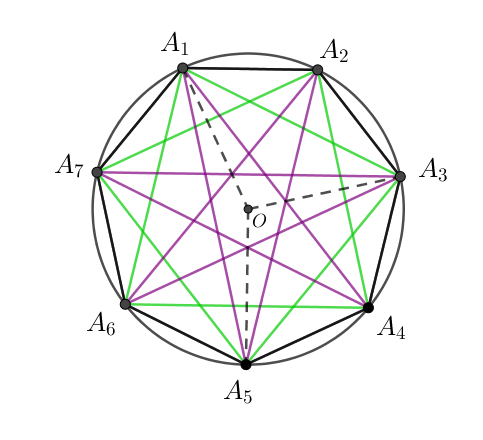
\includegraphics[scale=0.35]{38.PNG}
\end{figure}
Всего 2 вида диагоналей: 7 зеленых и 7 фиолетовых. Посчитаем квадрат зеленой:\\
$\Delta A_1 O A_3: A_1 A_3^2 = 1+1+2\cos{\frac{4\pi}{7}}=2(1+\cos{\frac{4\pi}{7}})$\\
$7A_1 A_3^2 = 14(1+\cos{\frac{4\pi}{7}})$\\
Квадрат фиолетовой:\\
$\Delta A_1 O A_5: A_1 A_5^2 = 1+1+2\cos{\frac{6\pi}{7}}=2(1+\cos{\frac{6\pi}{7}})$\\
$7A_1 A_5^2 = 14(1+\cos{\frac{6\pi}{7}})$\\
$Sum = 28 +14\cos{\frac{6\pi}{7}}+ 14\cos{\frac{6\pi}{7}}  $

%39 done
\item Докажите, что число $\frac{2+i}{2 - i}$ не является корнем $n$-ой степени из единицы ни для какого натурального $n$.

\textbf{Решение:} \\
$\frac{2 + i}{2 - i} = \frac{3 + 4i}{5}$\\
Пусть является, тогда $(\frac{3}{5} + \frac{4}{5}i)^n = 1 \\
1^n (\cos{(\arccos{3/5})} + \sin{(\arcsin{4/5})}) = 1 = 1 + 0i = \cos{0} + \sin{0} i
$ \\
Такого быть не может


\end{enumerate}

\subsection*{5. Кольца и поля}

\begin{enumerate}[resume]


%40 done
\item \textit{Полем из трёх элементов} называется множество из трёх элементов (обозначим их через 0, 1 и 2) с операциями сложения и умножения, заданными следующими таблицами:

\begin{minipage}{0.3\textwidth}

\begin{tabular}{ | l || l | l | l | }
\hline
$+$ & 0 & 1 & 2       \\ \hline \hline
0 & 0 & 1 & 2       \\ \hline
1 & 1 & 2 & 0    \\ \hline
2 & 2 & 0 & 1      \\
\hline
\end{tabular}
\end{minipage}
\begin{minipage}{0.3\textwidth}
\begin{tabular}{ | l || l | l | l | }
\hline
$\cdot$ & 0 & 1 & 2       \\ \hline \hline
0 & 0 & 0 & 0       \\ \hline
1 & 0 & 1 & 2    \\ \hline
2 & 0 & 2 & 1      \\
\hline
\end{tabular}
\end{minipage}

Проверьте ассоциативность и дистрибутивность этих операций. Проверьте, что из каждого элемента можно вычесть любой другой элемент, и каждый элемент можно поделить на любой другой ненулевой элемент.

СЛИШКОМ ИЗИ ЧТОБ РЕШАТЬ СОРИ

%41 done
\item (a) Рассмотрим множество $\bb{Z}/ 5\bb{Z}$ остатков $0,1,2,3,4$ при делении на $5$. Введем на $\bb{Z}/ 5\bb{Z}$ операции сложения и умножения с помощью следующих правил:
$$a+b = (a+b)\pmod{5},$$
$$ab=ab\pmod{5},$$
где сложение и умножение в правой части совпадают со сложением и умножением в $\bb{Z}$. Какие из аксиом поля выполняются для этих операций?\\
(б) Тот же вопрос для  $\bb{Z}/ 4\bb{Z}$
См.Лекции



%42 done
\item Пусть в поле $\bb{F}$ выполнено тождество $1+1 = 0$. Докажите или опровергните: уравнение  $$\underbrace{x + x + \ldots + x}_{n} = a$$ будет иметь единственное решение в поле $\bb{F}$ для любого элемента $a$ из поля и любого нечетного натурального $n$.

\textbf{Решенеие:}
\\
$1+1 = 0 \Longrightarrow a+a = 0, \text{так как} (1+1)a = 0\cdot a = a+a$\\
$x+x+...+x = a \Longrightarrow x = a$\\
\textbf{Ответ: } $x=a$



%43 done
\item Пусть в поле $\bb{F}$ тождество  $\underbrace{1 + 1 + \ldots + 1}_{n} = 0$  не выполнено ни для какого натурального $n$. Докажите или опровергните: уравнение 
$$\underbrace{x + x + \ldots + x}_{n} = a$$ 
будет иметь единственное решение в поле $\bb{F}$ для любого элемента $a$ из поля и любого натурального $n$.

\textbf{Решенеие:}
\\
Пусть $x+x+...+x = a = y+y+...+y \Longrightarrow (x-y)+(x-y)+...+(x-y)=0 \Longrightarrow (x-y)(1+1+...+1) = 0 \Longrightarrow x = y$ \text{ЧТД}


%44 done
\item (Единственность нуля). Докажите, что в кольце не может быть двух различных нулевых элементов, то есть элементов 0, для которых выполнено тождество $0 + a = a$. Доказательство должно опираться только на аксиомы кольца.

\textbf{Лемма.} Пусть в кольце $(L,+,\odot)$ есть нулевой элемент $O_{L}$. Тогда $\forall x \in L\colon 0_L \odot x = 0_L = x\odot 0_L$.

\textbf{Доказательство:}

По определению 0 имеем, что $0_L + O_L = 0_L$

Тогда $x\odot(0_L + O_L) = x\odot 0_L$

По дистрибутивности получим: $(x\odot0_L) + (x\odot0_L) = x\odot 0_L$

Прибавим справа ноль: $(x\odot0_L) + (x\odot0_L) = x\odot 0_L + 0_L$

Получим: $x\odot0_L = 0_L$

По аналогии можно доказать, что $0_L\odot x = 0_L$

Теперь докажем, что нуль в кольце единственен (решим саму задачу).

Предположим, что существует два нуля в кольце: $0$ и $0'$.

Тогда согласно доказанной лемме в кольце верно следующее:

$0'\odot0 = 0$\\
$0'\odot0 = 0'$\\
Тогда $0 = 0'\odot0 = 0' \Longleftrightarrow 0 = 0'$. Значит, нуль единственен в кольце, ч.т.д.

%45 done

\item Докажите, что в каждом кольце выполняются тождества
$$\text{а) } a\cdot 0 = 0 \quad \text{б) } -a = (-1)\cdot a \quad \text{в) } (-a)\cdot b = (-ab)$$

А, пункт а) был доказан в задаче 44 в виде леммы, а пункты б) и в) остаются в качестве упражнения.


%46 done
\item (Делители нуля). а) Докажите, что если
$$ab = 0$$
для двух элементов $a$ и $b$ поля, то либо $a = 0$, либо $b = 0$.

\textbf{Доказательство.}

Если $a = 0$, то условие выполнено. Теперь рассмотрим $a \neq 0$. Тогда по аксиоме поля для $a$ существует обратный ему элемент $a^{-1}$ такой, что $a^{-1}a = 1$. Умножим обе части равенства на $a^{-1}$. Получим 
$$a^{-1}(ab) = a^{-1}\cdot 0$$
По ассоциативности в поле заметим, что $a^{-1}(ab) = (a^{-1}a)b$, но т.к. $a^{-1}a = 1$, то $(a^{-1}a)b = 1b$. И по еще одной аксиоме $1b = b$. Значит, левая часть полученного равенства равна $b$. Но при этом правая часть по аксиомам равна $0$, т.к. $\forall x \quad 0\cdot x = x\cdot 0 = 0$ (хотя это, в общем-то, следствие из аксиом). Значит, $b = 0$. То есть из $ab= 0$ следует, что либо $a = 0$, либо $b = 0$, что и требовалось доказать.


(б) Приведите пример кольца, в котором есть делители нуля, то есть, два ненулевых элемента $a$ и $b$, такие что $ab = 0$.

\begin{minipage}{0.3\textwidth}
%\begin{flushleft}
$\bb{Z}/4$.
\begin{tabular}{ | l || l | l | l | l | }
\hline
. & 0 & 1 & 2 & 3      \\ \hline \hline
0 & 0 & 0 & 0 & 0      \\ \hline
1 & 0 & 1 & 2 & 3      \\ \hline
2 & 0 & 2 & 0 & 2      \\ \hline
3 & 0 & 3 & 2 & 1      \\
\hline
\end{tabular}
\\\\
Действительно, $2\cdot 2 = 0$
%\end{flushleft}
\end{minipage}
\begin{minipage}{0.5\textwidth}
%\begin{flushright}
Еще пример: $\bb{Z}/6$
\begin{tabular}{ | l || l | l | l | l | l | l | }
\hline
. & 0 & 1 & 2 & 3 & 4 & 5   \\ \hline \hline
0 & 0 & 0 & 0 & 0 & 0 & 0   \\ \hline
1 & 0 & 1 & 2 & 3 & 4 & 5   \\ \hline
2 & 0 & 2 & 4 & 0 & 2 & 4   \\ \hline
3 & 0 & 3 & 0 & 3 & 0 & 3   \\ \hline
4 & 0 & 4 & 2 & 0 & 4 & 2   \\ \hline
5 & 0 & 5 & 4 & 3 & 2 & 1   \\
\hline
\end{tabular}
\\\\
 Действительно, $2\cdot 3 = 0$.
%\end{flushright}
\end{minipage}


\end{enumerate}

\subsection*{6. Группы движений и перестановок}

\begin{enumerate}[resume]

%47 done
\item а) Разложите перестановку 
$$\sigma = 
\begin{pmatrix} 
1 & 2 & 3 & 4 & 5 & 6 & 7 & 8 & 9 \\
3 & 4 & 5 & 6 & 7 & 8 & 1 & 2 & 9
\end{pmatrix}
$$
в произведение непересекающихся циклов.

\textit{в условии, скорее всего, ошибка, потому исправлено на 9 переходит в 9}\\

\textbf{Решение:}

Проследим за 1: $1 \rightarrow 3 \rightarrow 5 \rightarrow 7 \rightarrow 1$. Получили цикл $(1, 3, 5, 7)$

Проследим за каким-нибудь оставшимся элементом, не вошедшим в первый цикл, например, за двойкой: $2 \rightarrow 4 \rightarrow 6 \rightarrow 8 \rightarrow 2$. Получили цикл $(2, 4, 6, 8)$

Остался элемент $9$, который переходит сам в себя, поэтому формально это цикл $(9)$, но его обычно не пишут.

Тогда $\sigma = (1, 3, 5, 7)(2, 4, 6, 8) $

б) Найдите знак перестановки $\sigma$.\\
\textbf{Решение:}\\
\textbf{Предложение 1. } Любой цикл представляется в виде произведения транспозиций, причем такое разложение можно указать явно:

$(i_1,i_2,\ldots i_k) = (i_1 i_2)(i_2 i_3)\ldots(i_k-1 i_k)$.

В частности, любая перестановка раскладывается в произведение транспозиций.

Пусть $\sigma = \tau_1\tau_2\ldots\tau_k$ - произвольное разложение перестановки $\sigma$ в произведение транпозиций $\tau_i$.

Тогда \textit{знаком} перестановки называется $sgn\sigma = (-1)^k$. Если число $k$ транспозиций четно, то $sgn\sigma = 1$ и перестановка называется \textit{четной}. Иначе, для нечетного кол-ва транспозиций $sgn\sigma = -1$ и перестановка называется нечетной.

\textbf{Следствие 1}. Транспозиции - нечетные перестановки.

\textbf{Следствие 2}. Четность цикла длины $k$ равна $-1^{k - 1}$

$sgn\sigma = (-1)^{4-1}\cdot(-1)^{4-1} = 1$.

в) Вычислите $\sigma^{2018}$\\
\textbf{Решение:}\\
Заметим из п.а), что $\sigma = (1, 3, 5, 7)(2, 4, 6, 8)$. Это значит, что $\sigma^4 = id$, поскольку композиция четырех $\sigma$ закольцует циклы и получится тождественное (проверьте непосредственно ручками). Тогда

$$\sigma^{2018} = (\sigma^{4})^{504}\sigma^2 = id^{507}\sigma^2 = \sigma^2 = \begin{pmatrix} 
1 & 2 & 3 & 4 & 5 & 6 & 7 & 8 & 9 \\
5 & 6 & 7 & 8 & 1 & 2 & 3 & 4 & 9
\end{pmatrix}
$$



%48 done
\item (а) Опишите все перестановки в $S_n$, которые могут быть разложены в произведение (возможно пересекающихся) циклов длины три.\\
\textbf{Решение:}\\
Тут надо написать, что циклы длины 3 порождаются двумя транспозициями, а это значит, что в перестановке $A \subset S_n$ должно быть четное число транспозиций, чтобы каждая пара "схлопнулась" в цикл длины 3. То есть это все такие четные перестановки. (нужно доработать решение).

(б) При каких $k$ в группе $S_n$ найдется перестановка с числом инверсий равным $k$?\\
\textbf{Решение:}\\
Сначала докажем, что максимальное число инверсий для перестановки $S_n \leq \frac{n(n-1)}{2}$. Докажем это с помощью индукции.

1. База. При $n = 1$ получаем перестановку без инверсий.

2. Шаг. Пусть верно для $n$. Докажем для $n+1$:

Для первых $n$ элементов в $S_{n+1}$ получим не больше $\frac{n(n-1)}{2}$ инверсий по предположению индукции. Для последнего $n+1$ элемента максимальное число инверсий равно $n$ (очевидно). Тогда суммарно всего инверсий не более чем $\frac{n(n-1)}{2} + n = \frac{n(n+1)}{2}$. Шаг доказан. Значит, утверждение верно для любого $n$.

Докажем точность оценки. Приведем пример перестановки, для которой число инверсий равно в точности $\frac{n(n-1)}{2}$: это перестановка 
$$
\sigma =
\begin{pmatrix} 
1 & 2   & \ldots & n -1 & n\\
n & n-1 & \ldots & 2    & 1
\end{pmatrix}
$$

Значит, при $k > \frac{n(n-1)}{2}$ в $S_n$ перестановки ровно с $k$ инверсиями не найдется. При $k = \frac{n(n-1)}{2}$ мы предъявили непосредственно перестановку $\sigma$. При $k < \frac{n(n-1)}{2}$ в $S_n$ найдется перестановка ровно с $k$ инверсиями (нужно построить непосредственно самостоятельно).

%49 done
\item (a) Опишите все повороты и отражения в группе симметрий правильного n-угольника при $n\geq2$ (эта группа называется группой диаэдра и обозначает $D_n$).\\
(б)Занумеруем вершины правильного n-угольника числами от $1$ до $n$ против часовой стрелки. Используя эту нумерацию, сопоставьте каждому движению из $D_n$ перестановку из $S_n$. Каким перестановкам из $S_n$ соответствуют повороты и отражения из пункта (а)? Чему равны знаки этих перестановок?\\
(в) При каких n отображение $D_n \longrightarrow S_n$ из пункта (б) является-взаимно-однозначным? Инъективным? Сюръективным?\\
\textbf{Решение:}

а) Для четного n можно заметить, что поворотов у нас n (id + сдвиг циклический, таких n-1), симметрии проходят через середины противоположных отрезков (между соседними вершинами) таких $\frac{n}{2}$ и через противоположные вершины таких тоже $\frac{n}{2}$ $\Rightarrow$ всего 2n.
Для нечетного n можно заметить, что поворотов тоже n, симметрии проходят через вершину и противоположную сторону $\Rightarrow$ таких n. Всего 2n.

Ответ 2n

б)????????????

в) Равны при n=3, ибо $D_3 = 6, S_3 = 6$, Инъективным при n>3, сюръективным при n<3

%50 done
\item (а) Докажите, что группа симметрий правильного тетраэдра изоморфна $S_4$.\\
(б) Какие перестановки вершин тетраэдра можно получить с помощью вращений тетраэдра?\\
(в)Докажите, что группа вращений правильного тетраэдра изоморфна $A_4$.\\
\textbf{Решение:}\\
a) $S_4 = 4!=24$ Группа симметрий правильного тетраэдра - переместить 1 вершину у нас 4 варианта, каждая вершина соединина с тремя другими $\Rightarrow$ есть 3! вариантов переместить оставшиеся вершины $\Rightarrow$ $4\cdot 3!=4!=24$ ЧТД\\
б) Вращение тетраэдра - это цикл из 3 элементов. Такой цикл состоит из 2 перестановок $\Rightarrow$ все перестановки $A_4$ можно получить вращением тетраэдра. \\
в) ТОЖЕ САМОЕ ЧТО И В ПУНКТЕ Б



%51
\item (а) Какие перестановки пространственных диагоналей куба можно получить с помощью вращений куба?\\
(б)Докажите, что группа вращений куба изоморфна $S_4$\\
\textbf{Решение:}\\
a) 





%52 done 
\item
а) Придумайте такое сюрьективное отображение $f:S_4->S_3$, чтобы для любых двух перестановок выполнялось тождество $f({\sigma_1}\cdot{\sigma_2})={f(\sigma_1)}\cdot{f(\sigma_2)}$\\
\textbf{Решение:}\\
Рассмотрим такие пары ребер тетраэдра, что в каждой паре ребра не являются соседними. Таких пар три. Каждое движение тетраэдра задает перестановку этих трех пар. В свою очередь, каждое движение тетаэдра задается перестановкой его вершин. \\
Композиция движений соответствует композиции перестановок пар несоседних ребер.\\
б) Найдите прообраз единичной перестановки\\
\textbf{Решение:}\\
Прообразом единичной перестановки будут те перестановки, которые каждую пару ребер переводит в себя (возможно, меняя ребра в какой-то паре местами).\\
Такими перестановками будут непересекающиеся пары транспозиций.




%53
\item (а) Пусть $G$ - конечная подгруппа группы движений плоскости. Докажите, что все элементы $g\in G$ имеют общую неподвижную точку $x$( то есть $g(x) = x$ для каждого $g\in G$).\\
(б) Классифицируйте все конечные подгруппы в группе движений плоскости.\\
\textbf{Решение:}





%54
\item Докажите изоморфизм групп 
$$GL_2({\bb{F}}_{2})\simeq S_3$$\\
\textbf{Решение:}

%55
\item Существует ли сюръективный гомоморфизм $S_4 \longrightarrow D_2$?\\
\textbf{Решение:}


\end{enumerate}

\subsection*{7. Многочлены}

\begin{enumerate}[resume]


%56 done
\item Примените решето Эратосфена, чтобы найти все неприводимые многочлены степени не выше четырех с коэффициентами в поле из 2 элементов.

\textbf{Решение:}

${1} ,\:\: {x} ,\:\: {x+1}\\
{x^2} ,\:\: {x^2+1} ,\:\: {x^2+x} ,\:\: {x^2+x+1},\\
{x^3} ,\:\: {x^3+1} ,\:\: {x^3+x} ,\:\: {x^3+x+1},\\
{x^3+x^2}, \:\:{x^3+x^2+1} ,\:\: {x^3+x^2+x} ,\:\: {x^3+x^2+x+1} ,\\
{x^4},\:\:  {x^4+1} ,\:\: {x^4+x} ,\:\: {x^4+x+1} ,\:\: {x^4+x^2} ,\:\: {x^4+x^2+1} ,\:\: {x^4+x^2+x},\\
{x^4+x^2+x+1} ,\:\: {x^4+x^3} ,\:\: {x^4+x^3+1} ,\:\: {x^4+x^3+x} ,\:\: {x^4+x^3+x+1} \\
{x^4+x^3+x^2} ,\:\: {x^4+x^3+x^2+1} ,\:\: {x^4+x^3+x^2+x} ,\:\: {x^4+x^3+x^2+x+1}$
Заметим, что многочлены с четным кол-вом элементов приводимые (подставим х=1 и получим 0), а остальные мы раскладываем. Значит неприводимые это х, х+1, $х^2+х+1$, $x^3+x+1$, $x^3+x^2+1$, $x^4+x+1$, $x^4+x^3+1$, $x^4+x^3+x^2+x+1$




%57 ???????
\item (а) Докажите для любого заданного поля $\bb{F}$, что существует бесконечно много неприводимых многочленов со старшими коэффициентами 1 и отсальными коэффициентами из $\bb{F}$.

\textbf{Решение:}
Пусть существует конечное число неприводимых функций над полем $\bb{F}$ : $f_1(x)$,\: $f_2(x)$\:...$f_{n-1}(x)$,\:$f_n(x)$. Перемножим все и прибавим 1.

$f_1(x)\cdot  f_2(x)\cdot \ldots f_{n-1}(x)\cdot f_{n}(x) +1 = g(x)$. Заметим, что $g(x)$ не делится на $f_i(x)$, где $i=1,2,3\ldots (n-1),n$, иначе 1 $\:\vdots \: f_i(x) \Rightarrow$ многочлен $g(x)$ неприводим над полем $\bb{F}$.

(б) Классифицируйте все неприводимые многочлены над $\bb{R}$ и над $\bb{С}$. (Подсказка: используйте основную теорему алгебры)

\textbf{Решение:}
По ОТА у многочленов над $\bb{С}$ неприводимые только многочлены 1 степени.

Неприводимыми над полем $\bb{R}$ многочлены первой степени и многочлены с дискрименантом меньше 0.\\
Возьмем некоторый непроводимый многочлен на $\bb{R}[x]$, тогда следуя первому утверждению у него имеется комплексный корень $ \alpha_{1} =a+b*i$, кроме того тогда его корнем также является  $\alpha_{2} =a-b*i$,следовательно многочлен делится на многочлены $(x-\alpha_{1})$ и $(x-\alpha_{2})$. Тогда многочлен делится также и на $(x-\alpha_{2})*(x-\alpha_{1})$
\begin{align*}
(x-\alpha_{2})*(x-\alpha_{1})=x^{2}-(\alpha_{1}+\alpha_{2})*x+\alpha_{1}*\alpha_{2}\\
x^{2}-(\alpha_{1}+\alpha_{2})*x+\alpha_{1}*\alpha_{2}=x^2-2*a*x+a^{2}+b{2}
\end{align*}
Получили противоречие, т.к. непреводимый многочлен делится на другой многочлен, отличный от себя.
Следовательно каждый многочлен можно разбить на непреводимые многочлены со степенью 2, и если имеются корни в рациональных числах то в разложении на непреводимые многочлены также будут присутсвовать многочлены степени 1.

%КАК ДОКАЗАТЬ Я НЕ ЕБУ СОРЯН
%Зато я ебу)

(в) Приведите пример неприводимого многочлена степени  5 над полем из двух элементов

\textbf{Решение:}
$x^5 + x + 1$\\
(г)Докажите, что над полем из двух элементов существует неприводимый многочлен любой заданной степени\\
\textbf{Решение:}

%58 done
\item Разложите на неприводимые множетели в $\bb{Q_{[x]}}$ многочлен $x^4 + 4x^3+x+6$

\textbf{Решение:}
$x^4 + 4x^3+x+6=(x^2-x+3)(x^2+x+2)$ 


\end{enumerate}

\subsection*{8. Целые гауссовы числа}

\begin{enumerate}[resume]

%59 done
\item Разложите 30 на простые множители в кольце целых гауссовых чисел.

\textbf{Решение:}
$30=2\cdot3\cdot5 = 3\cdot{(1-{i})\cdot(1+{i})}\cdot{(2-{i})(2+{i})}$

%60 done
\item Какие из простых чисел 2, 3, 5, 7, 11, 13, 17, 19, 23, 29 останусться простыми в кольце $\bb{Z}_{[i]}$?\\

\textbf{Решение:}
Числа 3, 7, 11, 19, 23 нельзя представить ввиде суммы двух квадратов $\Rightarrow$ они простые. 

$2=(1-i)(1+i)\quad 5=(2-i)(2+i)\quad 13=(3-2i)(3+2i)\quad 17=(1-4i)(1+4i)\quad 29=(5-2i)(5+2i)$


%61 
\item Пусть $\gamma$	- целое гауссово число. Введем отношение эквивалентности ${\thicksim}_{\gamma}$ на $\bb{Z}[i]$ по правилу $z{\thicksim}_{\gamma}\ \omega$, если $z - \omega$ делится на $\gamma$.\\
(а) Нарисуйте по одному представителю для каждого класса эквивалентности при $\gamma = 2\text{, }3 \text{ и } 5$.\\
(б)Найдите число классов эквивалентоности при $\gamma = 3-2i$.\\
\textbf{Решение:}

\end{enumerate}

\subsection*{9. Матрицы и системы линейных уравнений}

\begin{enumerate}[resume]

%62 done
\item
Вычислите $$\left(
\begin{array}{cc}
1 & 1\\
0 & i 
\end{array}
\right)$$

для всех натуральных $n$.

\textbf{Решение:}

Запомним мантру для умножения матриц: "строчки-столбцы. строчки-столбцы. строчки-столбцы". Повторяйте ее каждый раз перед сном и перед каждой парой по геометрии.

$A =\left(
\begin{array}{cc}
1 & 1\\
0 & i 
\end{array}
\right)$

$A^2 = \left(
\begin{array}{cc}
1 & 1\\
0 & i 
\end{array}
\right)\left(
\begin{array}{cc}
1 & 1\\
0 & i 
\end{array}
\right) = 
\left(
\begin{array}{cc}
1\cdot 1 + 1\cdot0 & 1\cdot 1 + 1\cdot i\\
0\cdot 1 + i\cdot 0 & 0\cdot1 + i\cdot i 
\end{array}
\right) = 
\left(
\begin{array}{cc}
1 & 1 + i\\
0 & -1 
\end{array}
\right)
$

$A^3 = A^2\cdot A = \left(
\begin{array}{cc}
1 & 1 + i\\
0 & -1 
\end{array}
\right)\cdot\left(
\begin{array}{cc}
1 & 1\\
0 & i 
\end{array}
\right) = \left(
\begin{array}{cc}
1 & 1 + i + i^2\\
0 & -1\cdot i 
\end{array}
\right)=
\left(
\begin{array}{cc}
1 & i\\
0 & -i 
\end{array}
\right)$

$A^4 = A^3\cdot A = \left(
\begin{array}{cc}
1 & i\\
0 & -i 
\end{array}
\right)\cdot\left(
\begin{array}{cc}
1 & 1\\
0 & i 
\end{array}
\right) = \left(
\begin{array}{cc}
1 & 1 + i^2\\
0 & -i^2 
\end{array}
\right) = \left(
\begin{array}{cc}
1 & 0\\
0 & 1 
\end{array}
\right) $ 

Круто, единичная матрица!

$A^5 = A^4\cdot A = e\cdot A = A$
Отлично!
Получили зацикливание, дальше все будет повторяться по тому же сценарию.

\textbf{Ответ:}

$A^n = \left(
\begin{array}{cc}
1 & 1\\
0 & i 
\end{array}
\right) \text{ при } n = 1 + 4k, \: k \in \N_{+0}$

$A^n = \left(
\begin{array}{cc}
1 & 1 + i\\
0 & -1 
\end{array}
\right) \text{ при } n = 2 + 4k, \: k \in \N_{+0}$

$A^n = \left(
\begin{array}{cc}
1 & i\\
0 & - i 
\end{array}
\right) \text{ при } n = 3 + 4k, \: k \in \N_{+0}$

$A^n = \left(
\begin{array}{cc}
1 & 0\\
0 & 1 
\end{array}
\right) \text{ при } n = 4k, \: k \in \N_{+0}$

%63 done
\item Приведите к стандартному ступенчатному виду "таблицу умножения", то есть, матрицу 10х10, у которой на (i,j)-том месте стоит ij

\textbf{Решение:}

$\begin{pmatrix} 
1 & 2 & 3 & 4 & 5 & 6 & 7 & 8 & 9 & 10 \\
2 & 4 & 6 & 8 & 10 & 12 & 14 & 16 & 18 & 20\\
3 & 6 & 9 & 12 & 15 & 18 & 21 & 24 & 27 & 30\\
4 & 8 & 12 & 16 & 20 & 24 & 28 & 32 & 36 & 40\\
5 & 10 & 15 & 20 & 25 & 30 & 35 & 40 & 45 & 50\\
6 & 12 & 18 & 24 & 30 & 36 & 42 & 48 & 54 & 60\\
7 & 14 & 21 & 28 & 35 & 42 & 49 & 56 & 63 & 70\\
8 & 16 & 24 & 32 & 40 & 48 & 56 & 64 & 72 & 80\\
9 & 18 & 27 & 36 & 45 & 54 & 63 & 72 & 81 & 90\\
10 & 20 & 30 & 40 & 50 & 60 & 70 & 80 & 90 &100
\end{pmatrix} \: \Rightarrow \begin{pmatrix} 
1 & 2 & 3 & 4 & 5 & 6 & 7 & 8 & 9 & 10 \\
0 & 0 & 0 & 0 & 0 & 0 & 0 & 0 & 0 & 0\\
0 & 0 & 0 & 0 & 0 & 0 & 0 & 0 & 0 & 0\\
0 & 0 & 0 & 0 & 0 & 0 & 0 & 0 & 0 & 0\\
0 & 0 & 0 & 0 & 0 & 0 & 0 & 0 & 0 & 0\\
0 & 0 & 0 & 0 & 0 & 0 & 0 & 0 & 0 & 0\\
0 & 0 & 0 & 0 & 0 & 0 & 0 & 0 & 0 & 0\\
0 & 0 & 0 & 0 & 0 & 0 & 0 & 0 & 0 & 0\\
0 & 0 & 0 & 0 & 0 & 0 & 0 & 0 & 0 & 0\\
0 & 0 & 0 & 0 & 0 & 0 & 0 & 0 & 0 & 0
\end{pmatrix}$



%64 done
\item Решите систему линейных уравнений 
$$
\begin{pmatrix} 
1 & 1 & 1 \\
1 & 2 & 3 \\
1 & 4 & 9
\end{pmatrix}
\begin{pmatrix} 
x \\
y \\
z
\end{pmatrix}
=
\begin{pmatrix} 
1  \\
2  \\
3 
\end{pmatrix}
$$

\textbf{Решение:}
$
\begin{cases}
   x+y+z=1 \quad (1) \\
   x+2y+3z=2\quad (2) \\
   x+4y+9z=3\quad (3)
 \end{cases}
$\\

$(2)-(1)\colon y+2z=1 \Longrightarrow y=1-2z$\\
$(3)-(2)\colon 2y+6z=1 \Longrightarrow 2(1-2z)+6z=1 \Longrightarrow z = -\frac{1}{2} \Longrightarrow y = 2$\\
$(1): x+2-\frac{1}{2}=1 \Longrightarrow x = -\frac{1}{2}$\\

\textbf{Ответ: } $(-\frac{1}{2}, 2, -\frac{1}{2})$


%65
\item a) Докажите, что если $m\times n$-матрица А получается из матрицы А' элементарными преобразованиями строк, то системы из m  однородных линейных уравнений по n неизвестных AX=0 и А'X=0 эквивалентны (то есть имеют одно и то же множесвто решений).
б) Сформулируцте и докажите аналогичное утверждение для систем неоднородных линейных уравнений.\\
\textbf{Решение:}




%66 done
\item Найдите линейную зависимость между строками матрицы 
$$
\begin{pmatrix} 
1 & 2 & 3 \\
2 & 3 & 6 \\
3 & 6 & 11 \\
2 & 5 & 8
\end{pmatrix}
$$

\textbf{Решение:}

$
\begin{cases}
   a_1+2a_2+3a_3+2a_4=0 \quad (1) \\
   2a_1+3a_2+6a_3+5a_4=0\quad (2) \\
   2a_1+2a_2+5a_3+8a_4=0\quad (3)
 \end{cases}
$\\

$2\cdot (1)-(2)\colon a_2 - a_4 = 0 \Longrightarrow a_2 = a_4$\\
$(3)- 3\cdot (1)\colon 2a_3 + 2a_4 = 0 \Longrightarrow a_3 = -a_4 = -a_2 $\\
$(1): a_1 + 2a_2 - 3a_2 + 2a_2 = 0 \Longrightarrow a_1 + a_2 =0 \Longrightarrow a_1 = -a_2 = a_3 $\\
Пусть $a_1 = 1 = a_3 \Longrightarrow a_2=a_4=-1 \Longrightarrow R_1 - R_2+R_3-R_4 = 0$\\
Ответ: $R_1 - R_2+R_3-R_4 = 0$




%67
\item Докажите, что если матрица $m\times n$ А' получается из матрицы А заменой i-ой строки на сумму i-той j-той строки, то $A'=(I_m +E_m^{i\cdot j})A$, где $I_m$ - единичная матрица $m\times m$- матрица, ${E_m}^{i\cdot j}$ - матрица того же размера с единственным ненклевым элементом (равным 1) на (i,j)-том месте.\\
\textbf{Решение:}\\



%68 done
\item Найдите матрицу обратную относительно умножения к матрице
$$\text{(а)} \begin{pmatrix} 
1 & 2 \\
2 & 3
\end{pmatrix},
\text{  (б)} \begin{pmatrix} 
1 & 2 & 3\\
2 & 3 & 6 \\
3 & 6 & 11
\end{pmatrix}
$$
\textbf{Решение:}\\
a)
$$\begin{pmatrix} 
1 & 2 \\
2 & 3
\end{pmatrix} \begin{pmatrix} 
1 & 0 \\
0 & 1
\end{pmatrix} \Rightarrow \begin{pmatrix} 
2 & 4 \\
2 & 3
\end{pmatrix} \begin{pmatrix} 
2 & 0 \\
0 & 1
\end{pmatrix} \Rightarrow \begin{pmatrix} 
0 & 1 \\
2 & 3
\end{pmatrix}\begin{pmatrix} 
2 & -1 \\
0 & 1
\end{pmatrix} \Rightarrow 
$$

$$\Rightarrow \begin{pmatrix} 
0 & 1 \\
2 & 0
\end{pmatrix}\begin{pmatrix} 
2 & -1 \\
-6 & 4
\end{pmatrix} \Rightarrow\begin{pmatrix} 
0 & 1 \\
1 & 0
\end{pmatrix}\begin{pmatrix} 
2 & -1 \\
-3 & 2
\end{pmatrix}
\Rightarrow \begin{pmatrix} 
1 & 0 \\
0 & 1
\end{pmatrix}\begin{pmatrix} 
-3 & 2 \\
2 & -1
\end{pmatrix}$$\\

\text{б)} $ \begin{pmatrix} 
1 & 2 & 3\\
2 & 3 & 6 \\
3 & 6 & 11
\end{pmatrix}\begin{pmatrix} 
1 & 0 & 0\\
0 & 1 & 0 \\
0 & 0 & 1
\end{pmatrix} \Rightarrow\begin{pmatrix} 
1 & 2 & 3\\
0 & -1 & 0 \\
0 & 0 & 2
\end{pmatrix}\begin{pmatrix} 
1 & 0 & 0\\
-2 & 1 & 0 \\
-3 & 0 & 1
\end{pmatrix} \Rightarrow\begin{pmatrix} 
1 & 0 & 3\\
0 & 1 & 0 \\
0 & 0 & 2
\end{pmatrix}\begin{pmatrix} 
-3 & 2 & 0\\
2 & -1 & 0 \\
-3 & 0 & 1
\end{pmatrix} \Rightarrow
$

$
\Rightarrow \begin{pmatrix} 
1 & 0 & 0\\
0 & 1 & 0 \\
0 & 0 & 1
\end{pmatrix}\begin{pmatrix} 
1,5 & 2 & -1,5\\
2 & -1 & 0 \\
-1,5 & 0 & 0,5
\end{pmatrix}
$

%69 done
\item а) При каком условии на коэффициенты $2\times 2$-матрица имеет  обратную?
б) тот же вопрос для $3\times 3$-матрицы.\\
\textbf{Решение:}
\\ а)$ \begin{vmatrix}
  a & b\\
  c & d
\end{vmatrix}  <=> ad - bc \neq 0$\\
б) $ \begin{vmatrix} 
      a_1 & a_2 & a_3 \\
      b_1 & b_2 & b_3 \\
      c_1 & c_2 & c_3
    \end{vmatrix} <=> a_1(b_2c_3 - b_3c_2) - b_1(a_2c_3 - a_3c_2) + c_1(a_2b_3 - a_3b_2)\neq 0  $


%70
\item Пусть А - квадратная матрица. Докажите, что следующие три условия эквивалентны.
1) Матрицу А можно перевести в единичную матрицу элементарными преобразованиями строк.
2) Матрица А имеет обратную относительно умножения.
3) Система линейных уравнений АХ=0 имеет только ненулевое решение.\\
\textbf{Решение:}


%71 done
\item Вычислите ранг матрицы
$$ \begin{pmatrix} 
11 & 12 & 13 & 14\\
21 & 22 & 23 & 24 \\
31 & 32 & 33 & 34 \\
41 & 42 & 43 & 44
\end{pmatrix}
$$
\textbf{Решение:}\\
$$ \begin{pmatrix} 
11 & 12 & 13 & 14\\
21 & 22 & 23 & 24 \\
31 & 32 & 33 & 34 \\
41 & 42 & 43 & 44
\end{pmatrix} \Rightarrow
\begin{pmatrix} 
11 & 12 & 13 & 14\\
10 & 10 & 10 & 10 \\
10 & 10 & 10 & 10 \\
10 & 10 & 10 & 10
\end{pmatrix} \Rightarrow
\begin{pmatrix} 
11 & 12 & 13 & 14\\
10 & 10 & 10 & 10\\
0 & 0 & 0 & 0\\
0 & 0 & 0 & 0
\end{pmatrix} \Rightarrow
\begin{pmatrix} 
11 & 1 & 1 & 1\\
10 & 0 & 0 & 0\\
0 & 0 & 0 & 0\\
0 & 0 & 0 & 0
\end{pmatrix} \Rightarrow
\begin{pmatrix} 
1 & 1 & 1 & 1\\
1 & 0 & 0 & 0\\
0 & 0 & 0 & 0\\
0 & 0 & 0 & 0
\end{pmatrix}
$$

$$
\Rightarrow
\begin{pmatrix} 
0 & 1 & 0 & 0\\
1 & 0 & 0 & 0\\
0 & 0 & 0 & 0\\
0 & 0 & 0 & 0
\end{pmatrix}\Rightarrow
\begin{pmatrix} 
1 & 0 & 0 & 0\\
0 & 1 & 0 & 0\\
0 & 0 & 0 & 0\\
0 & 0 & 0 & 0
\end{pmatrix}
$$\\

\text{Ранг матрицы = 2}

%72
\item Пусть $A$ и $B$ - матрицы размера $m\times n$ и $n\times k$ соответственно. Докажите неравенство на ранги:
$$rk(A+B)\leq min\{rk(A), rk(B)\}$$
\textbf{Решение:}


%73
\item Пусть $A$ и $B$ - квадратные матрицы. Докажите неравенство на ранги:
$$rk(A+B)\leq rk(A)+rk(B)$$
\textbf{Решение:}


%74 done ???????
\item Найдите число элементов в группе обратимых матриц $n\times n$ над полем из $p$ элементов\\
\textbf{Решение:}


%75 done
\item В десяти копилках лежат 1,2,3,...,10 момент. Разрешается добавлять по монете во все копилки, кроме одной. Можно ли, поворяя эту процедуру несколько раз, получить во всех копилках одинаковое число монет?\\
\textbf{Решение:}

%76
\item (а) На ребрах тетраэдра написаны числа $b_1, ..., b_6$. При каких условиях на эти числа можно написать еще $4$ числа на грани так, чтобы число на каждом из ребер оказалось равно сумме чисел, написанных на двух примыкающих к этому ребру гранях? Опишите все решения этой задачи для всех $b_1, ..., b_6$ для которых задача имеет решения.\\
(б)На вершинах куба написаны числа $b_1, ..., b_8$. При каких условиях на эти числа можно написать еще $6$ чисел на грани так, чтобы число на каждой из вершин оказалось равно сумме чисел, написанных на трех сходящихся в этой вершине гранях? Опишите все решения этой задачи для всех $b_1, ..., b_8$ для которых задача имеет решения.\\
\textbf{Решение:}

%77 done
\item Клетки прямоугольной таблицы заполнены числами так, что каждое число является средним арифметическим чисел в четырех соседних клетках (соседние = имеющие общую сторону). Можно ли восстановить числа во внутренних клетках таблицы по числам в граничных клетках?\\
\textbf{Решение:}

Пусть таблица $a\times b$ Да, так как возьмем клетку с координатами (2,1) (Левый нижний угол (0,0)). у нее известны 2 соседние клетки, она сама, одна пустая, а четвертая неизвество. по этим данным можно восстановить все клетки вида (х,0), (0,у), (x,b),(a,y). Далее двигаемся так же. УСЕЕЕ

%78
\item На табло горят несколько лампочек. Имеется несколько кнопок. Нажатие на кнопку меняет состояние лампочек, с которыми она соединена. Известно, что для любого набора лампочек найдется кнопка, соединенная с нечетным числом лампочек из этого набора. Докажите, что нажимая на кнопки, можно погасить все лампочки.\\
\textbf{Решение:}

%79
\item (а) В стаде $101$ корова. Если увести любую одну, то оставшихся можно разделить на два стада по $50$ коров в каждом, так что суммарный вес коров первого стада равен суммарному весу коров другого стада. Известно, что каждая корова весит целое число киллограммов. Докажите, что все коровы весят одинаково.\\
(б)Останется ли верно утверждение пункта (а) верным, если убрать условие, что вес коровы - целое число?\\
(в)Найдите ранг $(2n+1)\times (2n+1)$ матрицы, у которой на диагонали стоят нули, а все остальные коэффициенты равны либо $1$, либо $-1$, причем сумма коэффициентов в каждой строке равна нулю.\\
\textbf{Решение:}

\end{enumerate}

\subsection*{10. Векторные пространства}

\begin{enumerate}[resume]


%80 done
\item Докажите, что любые три вектора в $\bb{R}^2$ линейно зависимы.

\textbf{Решение:}
Пусть у нас есть векторы $u, w, v$. Если $u$ и $w$ лежат на одной прямой (коллинеарны), то задача решена. Иначе, они линейно независимы и порождают всю плоскость, тогда третий вектор будет выражаться как линейная комбинация двух других, т.е. векторы $u, w, v$ линейно зависимы.

Можно сказать и так: пусть векторы линейно независимы. Но т.к. их 3, а любой набор из $n$ линейно независимых векторов порождает $n$-мерное пространство $V$, то наши векторы порождают пространство с $\dim V = 3$, однако $\dim \R^2 = 2$.



%81 done
\item В $n$-мерном пространстве даны $n+2$ вектора $v_1, ..., v_{n+2}$. Докажите, что можно найти такие скаляры  ${\lambda}_{1}, ..., {\lambda}_{n+2}$ не равные одновременно нулю, что:
$$\lambda_{1}v_1+ \ldots +{\lambda}_{n+2}v_{n+2} =0, \ \ {\lambda}_{1} + \ldots + {\lambda}_{n+2} = 0 $$

\textbf{Решение:}

${\lambda}_{1} + \ldots + {\lambda}_{n+2} =0 \Longrightarrow \lambda_{n+2} = - \left(\lambda_1 + \lambda_2 + \ldots + \lambda_{n+1} \right)$

Тогда перепишем первое условие:
$$\lambda_{1}v_1+ \lambda_2 v_2 +  \ldots + \lambda_{n+1} v_{n+1} - \left(\lambda_{1} + \ldots + \lambda_{n+1}\right)v_{n+2} =0$$
$$\lambda_1(v_1 - v_{n+2}) + \lambda_2(v_2 - v_{n+2}) + \ldots + \lambda_{n+1}(v_{n+1} - v_{n+2}) = 0$$
$$\text{то есть } \lambda_1 u_1 + \ldots \lambda_n u_n + \lambda_{n+1} u_{n+1} = 0, \text{ где } u_k = v_k - v_{n+2} $$
Но любой набор из $(n+1)$ векторов в $n$-мерном пространстве заведомо линейно зависим, поэтому по определению линейной зависимости получим:
$$\exists \lambda_1, \lambda_ 2, \ldots, \lambda_{n+1} \neq 0 \text{ одновременно, такие что }\lambda_1 u_1 + \ldots + \lambda_n u_n + \lambda_{n+1} u_{n+1} = 0$$

То есть мы нашли такие $\lambda_1, \lambda_ 2, \ldots, \lambda_{n+1}$, что линейная комбинация векторов $v_1, v_2, \ldots, v_{n+2}$ тривиальна, что и требовалось по условию, осталось лишь вспомнить, что $\lambda_{n+2} = - \left(\lambda_1 + \lambda_2 + \ldots + \lambda_{n+1} \right)$, т.е. положим $\lambda_{n+2}$ согласно найденным $\lambda_1, \lambda_ 2, \ldots, \lambda_{n+1}$ и получим, что ${\lambda}_{1} + \ldots + {\lambda}_{n+2} = 0 $, что и требовалось.

%82 done
\item Какие из следующих подмножеств являются вещественными подпространствами в $\bb{R}[x]$ ?
$$(\text{а})\{f \ |\ f(1) =2\} \ \  \ (\text{б})\{f\ |\ f(1) = 0\} \ \ \ (\text{в})\{f\ |\ f  \text{ делится на } (x^2+1)\}$$
\textbf{Решение:}

Вспомним определение подпространства.

$\blacktriangleleft$ 

Непустое подмножество $L$ линейного пространства $V$ над полем $P$ называется \\ \textit{\textbf{линейным подпространством}}  пространства $V$, если

\begin{enumerate}
    \item $u + v \in L \quad \forall u, v \in L$ (подпространство замкнуто по отношению операции сложения);
    \item $\lambda\cdot v \in L \quad \forall v \in L \quad \forall \lambda \in P$ (подпространство замкнуто относительно умножения на скаляр)
\end{enumerate} 

Из определения подпространства следует, что нулевой вектор содержится в любом подпространстве. Действительно, возьмем $\lambda = 0$ и по второму пункту определения линейного подпространства получим, что $0\cdot v = 0 \in L$.

$\blacktriangleright$

Что такое $\bb{R}[x]$? Это пространство многочленов:
$$\bb{R}[x] = \{f \: | \: f(x) = a_0 + a_1x + a_2x^2 + ... + a_nx^n \ , \ a_0, ..., a_n \in \mathbb{R} \}$$

Теперь мы готовы решать задания.

а) Рассмотрим подмножество $\{f \ |\ f(1) =2\}$. 

$f(x) = a_0 + a_1x + a_2x^2 + ... + a_nx^n$

$2 = f(1) = a_0 + a_1\cdot 1 + a_2\cdot1^2 + \ldots + a_n\cdot1^n = a_0 + a_1 + a_2 + \ldots + a_n$

Это означает, что подмножество $\{f \ |\ f(1) =2\}$ содержит в себе все многочлены, сумма коэффицентов которых равна двум. Однако тогда понятно, что нулевой многочлен явно не принадлежит этому множеству, т.к. $0 = 0 + 0\cdot x + 0\cdot x^2 + \ldots + 0\cdot x_n$, то есть сумма его коэффициентов равна нулю. Значит, это подмножество не является подпространством по определению.

б) Рассмотрим подмножество $\{f \ |\ f(1) =0\}$. 

$f(x) = a_0 + a_1x + a_2x^2 + ... + a_nx^n$

$0 = f(1) = a_0 + a_1\cdot 1 + a_2\cdot1^2 + \ldots + a_n\cdot1^n = a_0 + a_1 + a_2 + \ldots + a_n$

Это означает, что подмножество $\{f \ |\ f(1) =0\}$ содержит в себе все многочлены, сумма коэффицентов которых равна нулю. Тогда проверим по определению, является ли это подмножество линейным подпространством:

\begin{enumerate}
    \item $u + v \in L \quad \forall u, v \in L$
    Действительно, пусть $f \in L, \: g \in L$, тогда
    
    $f(1) = a_0 + a_1\cdot 1 + \ldots + a_n\cdot 1^n, \quad a_0 + a_1 + \ldots + a_n = 0$
    
    $g(1) = b_0 + b_1\cdot 1 + \ldots + b_n\cdot 1^n, \quad a_b + b_1 + \ldots + b_n = 0$
    
    $(f + g)(1) = (a_0 + b_0) + (a_1 + b_1)\cdot 1+ (a_2 + b_2)\cdot 1^2 + \ldots + (a_n + b_n)\cdot 1^n = a_0 + b_0 + a_1 + b_1 + \ldots + a_n + b_n = 0 + 0 = 0$. Значит, $f + g \in L$
    
    \item $\lambda\cdot v \in L \quad \forall v \in L \quad \forall \lambda \in P$
    $f = a_0 + a_1\cdot x + \ldots + a_n\cdot x^n, \quad a_0 + a_1 + \ldots + a_n = 0$
    
    $f\cdot\lambda = a_0\lambda + a_1\lambda x + \ldots + a_n\lambda x^n$
    
    $\lambda f(1) = a_0\lambda + a_1\lambda + \ldots + a_n\lambda = \lambda\cdot(a_0 + a_1 + \ldots + a_n) = \lambda\cdot 0 = 0$
    
\end{enumerate}

Подмножество $\{f \ |\ f(1) =0\}$ является подпространством по определению.

в) Рассмотрим подмножество $\{f \ |\ f \text{ делится на } (x^2 + 1) \}$. 

Если $f$ делится на $(x^2 + 1)$, это значит, что $f = (x^2 + 1)\cdot Q_{n-2}(x)$, где $Q_{n-2}(x)$ - многочлен от $x$ степени $n - 2$.

Тогда понятно, что сумма таких многочленов также делится на $x^2 + 1$, то есть данное множество замкнутно относительно операции сложения.

И понятно, что при умножении на произвольный скаляр наш многочлен по-прежнему будет делиться на $(x^2 + 1)$, значит, по определению данное множество является подпространством.


%83
\item Какие из следующих подмножеств являются комплексными подпространствами в $\mathbb{C}^2$ ?
$$(\text{а})\{(x,y)\in\mathbb{C}^{2}\ |\ x\in\bb{R}\} \ \  \ (\text{б})\{(x,y)\in\mathbb{C}^{2}\ |\ x=y\}$$
\textbf{Решение:}

%84 done
\item Являются ли линейно зависимыми над $\bb{R}$ векторы
$$ \text{а)}(1,2,3),(1,2,4),(1,3,4) \in\bb{R}^3;\ \text{б)}(1,2,3,5),(2,3,5,8),(3,4,7,11) \in\bb{R}^4?$$

\textbf{Решение:}

а) $
\begin{cases}
   a_1+a_2+a_3=0 \quad (1) \\
   2a_1+2a_2+3a_3=0\quad (2) \\
   3a_1+4a_2+4a_3=0\quad (3)
 \end{cases}
$\\

$(2)-2\cdot(1)\colon a_3 = 0 $\\
$(1): a_1 + a_2 = 0 \Longrightarrow a_1 = -a_2$\\
$(3): 3a_1 + 4a_2 = 0 \Longrightarrow -3a_2+4a_2 = a_2 = 0 \Longrightarrow a_1=a_2=0=a_3$, \text{противоречие определению} $\Longrightarrow$ \text{не являются линейно зависимыми}\\
\textbf{Ответ: } \text{не являются}

б) $
\begin{cases}
   a_1+2a_2+3a_3=0 \quad (1) \\
   2a_1+3a_2+4a_3=0\quad (2) \\
   3a_1+5a_2+7a_3=0\quad (3) \\
   5a_1+8a_2+11a_3=0\quad (4)
 \end{cases}
$\\

$2\cdot (1)-(2)\colon a_2+2a_3 = 0 \Longrightarrow a_2 = -2a_3 $\\
$(3)-(2)\colon a_1+2a_2+3a_3 = 0 \Longrightarrow a_1-4a_3+3a_3 = 0 \Longrightarrow a_1 = a_3$\\
Пусть $a_1 = 1 = a_3 \Longrightarrow a_2= -2 \Longrightarrow R_1 - 2R_2+R_3 = 0$\\
\textbf{Ответ: } $R_1 - 2R_2+R_3 = 0$

%85 done
\item Постройте базис над $\bb{R}$ в пространстве всех кососимметрических $n\times n$-матриц с вещественными коэффициентами

\textbf{Решение:}
Кососимметрической матрицей $n\times n$ называется матрица $A$ вида
\[
A = 
\begin{pmatrix}
0       & a_{12}  & a_{13}  & \dots  & a_{1n} \\
-a_{12} & 0       & a_{23}  & \dots  & a_{2n} \\
-a_{13} & -a_{23} & 0       & \dots  & a_{3n} \\
\vdots  &         &         & \ddots & \vdots \\
-a_{1n} & -a_{2n} & -a_{3n} & \dots  & 0
\end{pmatrix}
\]
Заметим, что кососимметрическая матрица однозначно задается элементами выше(ниже) главной диагонали.

Построим следующий базис:

$e_{1,2} = 
\left(
\begin{smallmatrix}
0       & 1  & 0  & \dots  & 0 \\
-1 & 0       & 0  & \dots  & 0 \\
0 & 0  & 0  & \dots  & 0 \\
\vdots  &         &  & \ddots & \vdots \\
0 & -0 & 0 & \dots  & 0
\end{smallmatrix}
\right)
\quad 
\ldots,\quad  
e_{n-1, n}
\left(
\begin{smallmatrix}
0       & 0    & 0      & 0     \dots  & 0  \\
0       & 0    & 0      & 0     \dots  & 0 \\
0       & 0    & 0      & 0     \dots  & 0 \\
\vdots  &      &        &       \ddots & \vdots \\
0       & -0   & 0      &       \dots  & 1 \\
0       & -0   & \dots  & -1           & 0
\end{smallmatrix}
\right)
$

Где $e_{i,j} \:(i < j)$ -- матрица, у которой элемент $(i,j) = 1$, элемент $(j,i) = -1$, а остальные элементы - нули. Число таких матриц равно числу наддиагональных элементов кососимметрической матрицы размерности $n\times n \colon \frac{n(n-1)}{2}$. Достаточно очевидно, что матрицы $e_{1,2},\ldots e_{n-1, n}$ линейно независимы (попробуйте мысленно все $n^2$ элементов матриц записать в одну линию, тогда у каждого $e_{i,j}$ будут свои уникальные места-координаты, в которых они не равны 0). При этом любая кососимметрическая матрица представима в виде их линейной комбинации.

Действительно, 
$$A = 
\begin{pmatrix}
0       & a_{12}  & a_{13}  & \dots  & a_{1n} \\
-a_{12} & 0       & a_{23}  & \dots  & a_{2n} \\
-a_{13} & -a_{23} & 0       & \dots  & a_{3n} \\
\vdots  &         &         & \ddots & \vdots \\
-a_{1n} & -a_{2n} & -a_{3n} & \dots  & 0
\end{pmatrix} = 
a_{12}\cdot e_{12} + \ldots + a_{n-1, n}\cdot e_{n-1, n}$$.

Следовательно, $e_{1,2},\ldots e_{n-1, n}$ образуют базис пространства $M$ кососсиметрических матриц, причем $dim M = \frac{n(n-1)}{2}$.


%86 ???????????????????????????????????????????????
\item Можно ли представить $\sqrt[3]{4}$ как линейную комбинацию $a+b\sqrt[3]{2}$, где $a$ и $b$ - рациональные числа?

\textbf{Решение:}

$\sqrt[3]{4} = a+b\sqrt[3]{2}$ \text{возведем в куб}\\
$4 = a^3+3a^2 b\sqrt[3]{2} + 3ab^2\sqrt[3]{4} +2b^3$\\
$\Longrightarrow a = 0  \Longrightarrow 2b^3 = 4 \Longrightarrow b = \sqrt[3]{2}$ \text{- не рациональное} $\Longrightarrow$ \text{нельзя}\\
\textbf{Ответ: нельзя}






%87 done
\item Представлется ли многочлен $1+x+x^2+x^3$ \text{в виде линейной комбинации с вещественными} коэффициентами многочленов
$$ \text{а)} x+1, (x+1)^2, (x+1)^3;\ \text{б)} x-1, (x-1)^2, (x-1)^3?$$

\textbf{Решение:}

а)$x^3+x^2+x+1 = a_1(x+1) + a_2(x^2+ 2x+1) + a_3(x^3+3x^2+3x+1)$\\
$x^3+x^2+x+1 = a_1 x+a_1 + a_2 x^2 + 2a_2 x+a_2 + a_3 x^3+3a_3 x^2+3a_3 x+a_3$\\
$x^3+x^2+x+1 = a_3 x^3+(a_2+3a_3)x^2+(a_1+2a_2+3a_3)x+(a_1+a_2+a_3)$\\
$\Longrightarrow a_3 = 1$\\
$\Longrightarrow a_2+3a_3 = 1 \Longrightarrow a_2 + 3 = 1\Longrightarrow a_2 = -2$\\
$\Longrightarrow a_1+2a_2+3a_3 = 1 \Longrightarrow a_1 -4 + 3 = 1\Longrightarrow a_1 = 2$\\
$\Longrightarrow a_1+a_2+a_3 = 1 \Longrightarrow 2-2+1 = 1\Longrightarrow \text{верно}$\\
$\Longrightarrow$ \text{представляется} \\
\textbf{Ответ: } представляется $x^3+x^2+x+1 = 2(x+1) + -2(x+1)^2 + (x+1)^3$\\

б)$x^3+x^2+x+1 = a_1(x-1) + a_2(x^2- 2x+1) + a_3(x^3-3x^2+3x-1)$\\
$x^3+x^2+x+1 = a_1 x-a_1 + a_2 x^2 - 2a_2 x+a_2 + a_3 x^3-3a_3 x^2+3a_3 x-a_3$\\
$x^3+x^2+x+1 = a_3 x^3+(-2a_2-3a_3)x^2+(a_1-2a_2+3a_3)x+(-a_1+a_2-a_3)$\\
$\Longrightarrow a_3 = 1$\\
$\Longrightarrow -2a_2+3a_3 = 1 \Longrightarrow -2a_2 - 3 = 1\Longrightarrow a_2 = -2$\\
$\Longrightarrow a_1-2a_2+3a_3 = 1 \Longrightarrow a_1 +4 + 3 = 1\Longrightarrow a_1 = -6$\\
$\Longrightarrow -a_1+a_2-a_3 = 1 \Longrightarrow 6-2-1\neq 1\Longrightarrow \text{неверно}$\\
$\Longrightarrow$ \text{не представляется} \\
\textbf{Ответ: }\text{не представляется}

%88 done 
\item Пусть $\bb{V}$ - вещественное векторное пространство всех вещественных функций на отрезке [0,1].\\
а)Являются ли функции $x^3, \sin{x},\cos{x}$ и $e^x$ \text{линейно зависимыми в} $\bb{V}$?\\
б)Тот же вопрос для функций $1, \sin{^2} (x), \cos{^2}(x)$.

\textbf{Решение:}\\
a) $\lambda_1\cdot x^3 + \lambda_2 \cdot \sin{x}+\lambda_3\cdot\cos{x}+\lambda_4\cdot e^x=0$ Беру производную\\
$\lambda_1\cdot 3x^2 + \lambda_2 \cdot \cos{x}-\lambda_3\cdot\sin{x}+\lambda_4\cdot e^x=0\\
\lambda_1\cdot 6x - \lambda_2 \cdot \sin{x}-\lambda_3\cdot\cos{x}+\lambda_4\cdot e^x=0\\
\lambda_1\cdot 6 - \lambda_2 \cdot \cos{x}+\lambda_3\cdot\sin{x}+\lambda_4\cdot e^x=0\\
\lambda_2 \cdot \sin{x}+\lambda_3\cdot\cos{x}+\lambda_4\cdot e^x=0\\
\lambda_1\cdot 6x +2\lambda_4\cdot e^x=0\\
\lambda_1\cdot (3x^2+6) + 2\lambda_4\cdot e^x=0\\
\lambda_1\cdot (3x^2-6x+6) =0\\
3x^2-6x+6=0\\$
Нет решения для всех х $\Rightarrow$ Не линейно зависимы\\

б)\textbf{Ответ: } Да, являются, $\sin{^2} (x) + \cos{^2}(x) = 1 $



%89 done
\item Рассмотрим поле $\R$ как векторное пространство над $\Q$.\\
а) Являются ли линейно зависимыми векторы $1, \sqrt{2}, \frac{1}{\sqrt{2}-1}?$\\
б)Выразите вектор $\frac{1+\sqrt{2}}{3-2\sqrt{2}}$ \text{как линейную комбинацию} векторов $1 \text{ и } \sqrt{2}$.\\
в)Являются ли линейно зависимыми векторы $1, \sqrt[3]{2}, \frac{1}{\sqrt[3]{2}-1}?$\\
г)Можно ли выразить вектор $\frac{1}{\sqrt[3]{2}-1}$ \text{как линейную комбинацию} векторов $1,\sqrt[3]{2}, \sqrt[3]{4} $?

\textbf{Решение:}

а) $a_1+a_2 \sqrt{2} + a_3\frac{1}{\sqrt{2}-1} = 0$\\
$a_1+a_2 \sqrt{2} + a_3(\sqrt{2}+1) = 0$\\
$a_1+a_3 = -\sqrt{2}(a_3+a_2)$\\
Если $a_3 = -a_2 \Longrightarrow a_1-a_2 = 0 \Longrightarrow a_1 = a_2 = -a_3$\\
Пусть $a_1 = 1 \Longrightarrow a_2=1 \Longrightarrow a_3 = -1$
$\Longrightarrow 1+\sqrt{2} -\frac{1}{\sqrt{2}-1} = 0$\\
\textbf{Ответ: }\text{являются, } $1+\sqrt{2} -\frac{1}{\sqrt{2}-1} = 0$\\

б)$\frac{1}{\sqrt[3]{2}-1} = a_1 +a_2\sqrt{2}$\\
$(1+\sqrt{2})(3+2\sqrt{2}) = a_1+a_2\sqrt{2} $\\
$3+ 3\sqrt{2}+2\sqrt{2}+4 = a_1+a_2\sqrt{2} $\\
$7+5\sqrt{2} = a_1+a_2\sqrt{2} \Longrightarrow a_1 = 7, a_2 = 5$\\

\textbf{Ответ: }$\frac{1+\sqrt{2}}{3-2\sqrt{2}} = 7+5\sqrt{2}$\\

в)$a_1+a_2\sqrt[3]{2}+a_3\frac{1}{\sqrt[3]{2}-1} = 0$\\
$(\sqrt[3]{2}-1)a_1 + (\sqrt[3]{4}-\sqrt[3]{2})a_2 + a_3 = 0 $\\
$\sqrt[3]{2}a_1 + \sqrt[3]{4}a_2 - \sqrt[3]{2}a_2 -a_1+a_3=0$\\
Пусть $\sqrt[3]{2} =x \Longrightarrow x^2 a_2 + x(a_1+a_2)-a_1+a_3=0\cdot x^2 + 0\cdot x+ 0$
$\Longrightarrow a_2 = 0
\Longrightarrow a_1=a_2=0
\Longrightarrow a_3=a_1=a_2=0 \text{ противоречие определению} \Longrightarrow \text{не являются}$\\
\textbf{Ответ: }\text{не являются}

г)$\frac{1}{\sqrt[3]{2}-1} = a_1 + a_2\sqrt[3]{2}+a_3\sqrt[3]{4}$\\
$\sqrt[3]{4}+\sqrt[3]{2}+1 = a_1+a_2\sqrt[3]{2}+a_3\sqrt[3]{4} \Longrightarrow a_1=a_2=a_3 = 1$\\
\textbf{Ответ: }\text{можно, } $1+\sqrt[3]{2}+\sqrt[3]{4} = \frac{1}{\sqrt[3]{2}-1}$\\



%90
\item Чему равна размерность поля комплексных чисел, рассматриваемое как векторное пространство над полем
$$\text{(а) рациональных чисел; (б) вещественных чисел; (в)комплексных чисел?}$$
\textbf{Решение:}




%91
\item Пусть  $\bb{F}\subset\mathbb{C}$ - минимальное подполе, содержащее все корни многочлена $f(x)\in\bb{Q}[x]$. Найдите размерность поля $\bb{F}$ как векторного простарнства над $\bb{Q}$, если:
$$ (\text{а}) x^2-2; \ (\text{б}) x^3-2; \  \ (\text{в}) x^4+4; \ (\text{г}) x^4+1; \ (\text{д}) x^4-2$$
\textbf{Решение:}







%92 done
\item Пусть $\bb{F}_p$ - конечное поле из $q$ элементов. Найдите число всех подпространств в координатной плоскости $\bb{F}^2_q$.

\textbf{*Бонус от Андрея:} Решение задачи в общем виде для $k$-мерных подпространств векторного пространства $\bb{F}^n_q$.


\textbf{Решение:}
Вспомним, что такое подпространство $L$ некоторого линейного пространства $\bb{R}^n$:

Множество $L \subset \bb{R}^n$ называется подпространством $\bb{R}^n$, если

1) $\forall x, y \in L \quad x + y \in L$

2) $\forall x \in L, \lambda \in R \quad \lambda\cdot x \in L$

Заметим, что если $L$ состоит из единственного нулевого вектора, то это действительно линейное подпространство (\textit{тривиальное линейное подпространство размерности 0}). Действительно, $0 \in L \quad 0 + 0 \in L$ и $\lambda\cdot 0 = 0 \in L$.

По условию задачи необходимо найти все такие подпространства в координатной плоскости $\bb{F}^2_q$. То есть найти подпространства размерностей 0 и 1 и затем сложить их.
Мы уже знаем, что пространство размерности 0 одно и состоит в точности из нулевого вектора. Теперь найдем количество подпространств размерности 1.

Заметим, что всего векторов $v \in \bb{F}^2_q$ ровно $q^2$, поскольку каждая из двух координат может принимать любое значение из поля $\bb{F}_q$. 

Подпространство размерности 1 (прямая) задается единственным вектором. Из всех $q^2$ векторов мы должны выбрать любой ненулевой вектор, т.е. $q^2 - 1$ таких векторов. Но заметим, что коллинеарные векторы задают одно и то же подпространство (прямую), поэтому мы каждое подпространство посчитали $q - 1$ раз (столько коллинеарных ненулевых векторов лежат на одной прямой). Тогда подпространств размерности 1 всего $\frac{q^2 - 1}{q - 1} = q + 1$. А всего подпространств в координатной плоскости $\bb{F}^2_q$ получим $q + 2$. (Если не считать тривиальное, то получим $q + 1$). 

Теперь заодно решим более общую задачу, которой нет в листке для подготовки, но она достаточно полезна.


\textbf{*Задача.}
Требуется найти количество $k$-мерных подпространств в пространстве $\bb{F}^n_p$

Найдем количество векторов в $\bb{F}^n_p$. Поскольку размерность этого пространства равна $n$, то каждая из $n$ координат может принимать любое значение из поля $\bb{F}_p$, тогда всего векторов \\ $\underbrace{q\cdot q\cdot \ldots \cdot q}_{n} = q^n$. Теперь чтобы задать $k$-мерное подпространство, нам необходимо выбрать $k$ линейно независимых вектора, которые и будут порождать линейное подпространство размерности $k$. Первый вектор можено выбрать любой, кроме нулевого (поскольку нулевой вектор автоматически делает любую систему векторов линейно зависимой), т.е. $q^n - 1$ таких векторов. Второй вектор мы обязаны выбрать вне линейной оболочки первого вектора (первый вектор задает прямую, поэтому второй вектор необходимо выбрать не на этой прямой). Таких векторов ровно $q^n - q$. Проделаем такую операцию для всех оставшихся векторов и получим $$(q^n - 1)(q^n - q)\cdot\ldots\cdot(q^n - q^{k-1}) \quad (1)$$ способов выбрать $k$ линейно независимых векторов в пространстве $\bb{F}^n_p$.

Но теперь заметим, что существует много различных наборов из $k$ векторов, которые порождают одно и то же линейное подпространство. Простейший наглядный пример: ортогональные векторы $(x, y)$ и $(y, x)$ задают одну и ту же плоскость, то есть одно и то же подпространство мы посчитали дважды. Чтобы учесть это, посчитаем количество способов выбрать $k$ линейно независимых векторов в пространстве размерности $k$. Но мы это только что проделали чуть выше, нужно лишь заменить $n$ на $k$ в формуле (1). Получим $(q^k - 1)(q^k - q)\cdot\ldots\cdot(q^k - q^{k-1})$ различных базисов, задающих одно и то же линейное подпространство. Тогда количество $n$ различных $k$-мерных подпространств в пространстве $\bb{F}^n_p$ составляет ровно
$$n = \frac{(q^n - 1)(q^n - q)\cdot\ldots\cdot(q^n - q^{k-1})}{(q^k - 1)(q^k - 1)\cdot\ldots\cdot(q^k - q^{k-1})}$$

Осталось заметить, что если требуется найти количество \textbf{всех} линейных подпространств пространства $\bb{F}^n_p$, необходимо воспользоваться этой формулой при $k = 0, 1, 2, \ldots n-1$ и просуммировать количества всех подпространств размерностей $0, 1, \ldots n - 1$.

%93 done
\item (Формула Тейлора). Для каждого $a\in\bb{R}$ постройте базис в пространстве вещественных многочленов степени не выше $n$, так чтобы каждый многочлен $f$ в этом базисе имел координаты $(f(a), f'(a), ..., f^{(n)}(a))$\\
\textbf{Решение:}\\
Формула Тейлора: $P(x) = f(x_0) + \frac{f'(x_0)(x-x_0)}{1!}+...+\frac{f^(n)(x_0)(x-x_0)^n}{n!}$\\
Также: $P(x) = f(x_0)e_1+f'(x_0)e_2+...+f^(n) e_n$\\
$\Longrightarrow e_1 = 1, e_2=\frac{x-x_o}{1!}, ..., e_n = \frac{(x-x_0)^n}{n!}$


%94 done
\item (Интерполяционная формула Лагранжа). Для данного набора попарно различных точек $a_0, a_1, ..., a_n\in\bb{R}$ постройте базис в пространстве вещественных многочленов степени не выше $n$, так чтобы каждый многочлен $f$ в этом базисе имел координаты $(f(a_0), f(a_1), ..., f(a_n))$\\
\textbf{Решение:}\\
Интерполяционная формула Лагранжа: ${\sum}_{i=0}^n = y_i \frac{(a-a_0)(a-a_1)...(a-a_{i-1})(a-a_{i+1})...(a-a_n)}{(a_i-a_0)(a_i-a_1)...(a_i-a_{i-1})(a_i-a_{i+1})...(a_i-a_n)}$\\
$P(a) = f(a_0)e_1 + f(a_1)e_2 +...+ f(a_n)e_n$\\
$\Longrightarrow e_i = \frac{(a-a_0)(a-a_1)...(a-a_{i-1})(a-a_{i+1})...(a-a_n)}{(a_i-a_0)(a_i-a_1)...(a_i-a_{i-1})(a_i-a_{i+1})...(a_i-a_n)}$



%95 done
\item Пусть $U\subset \bb{F}^4_2$ - плоскость в 4-хмерном пространстве над полем из двух элементов. Найдите количество таких плоскостей $V\subset \bb{F}^4_2$, что $U\cap V =\{0\}$

\textbf{Решение:}

Посчитаем количество векторов в $\bb{F}^4_2$: их $2^4 = 16$, т.к. 4 координаты и каждая либо 0, либо 1. Теперь зафиксируем плоскость $U$ из условия: она порождается некоторыми двумя векторами. Пусть эти векторы $u$ и $v$. Тогда в плоскости $U$ лежат векторы $0, u, v, u + v$. 

Теперь, чтобы найти количество таких плоскостей $V\subset \bb{F}^4_2$, что $U\cap V =\{0\}$, нам необходимо выбрать 2 вектора, порождающих эту плоскость $V$ так, чтобы $U\cap V =\{0\}$. Но это означает, что из всех 16 векторов нам нельзя брать векторы $0, u, v, u + v$, иначе наши плоскости пересекутся не по нулю. Тогда для первого вектора, который будет порождать плоскость $V$, всего $16 - 4 = 12$ способов выбрать его. А для второго вектора нам необходимо выбрать любой, который не будет лежать в линейной оболочке первого, т.е. коллинеарен ему (но т.к. у нас пространство над полем из двух элементов, то таких векторов нет). Значит, для второго вектора у нас $12 - 1 = 11$ способов выбрать его. Тогда получим $12\cdot 11$ способов выбрать 2 линейно независимых вектора таких, что они породят подпространство размерности 2 (плоскость), пересекающуюся с зафиксированной по нулю. 

Но теперь заметим, что мы посчитали каждое подпространство (плоскость) дважды: действительно, пусть подпространство порождено векторами $a, b$, тогда оно так же порождено векторами $b, a$, поэтому итоговое количество плоскостей $V$ равно $\frac{12\cdot 11}{2} = 66$.

Ответ: $66$ плоскостей.



\end{enumerate}
\subsection*{11. Линейные операторы}

\begin{enumerate}[resume]


%96 done
\item (a)Покажите, что векторы $1$ и $i$ образуют базис в поле комплексных чисел, рассматриваемом как векторное пространство над $\bb{R}$\\
(б) Выпишите матрицу оператора умножения на комплексное число $a+bi$ в базисе $\{1, i\}$\\
\textbf{Решение:}\\
a) Пусть не образуют базис, тогда $\lambda_1\cdot 1 + \lambda_2\cdot i =0\\
i=-1\cdot \frac{\lambda_1}{\lambda_2}$
Но i не рациональное, а справа нашего равенства получилось рациональное число. ЧТД\\
б) Умножим базисные вектора на $a+bi$. $1\cdot (a+bi)=a+bi i\cdot (a+bi)= -b + ai$ Запишем в матрицу результаты $\begin{pmatrix} 
a & -b\\
b & a\\
\end{pmatrix}$

%97 done
\item Найдите два линейных оператора $T$ и $U$ на $\bb{R}^2$ такие, что $TU = 0$, но $UT \neq 0$.
\\
\textbf{Решение:}\\
Пример:
$T = 
\begin{pmatrix} 
0 & 1 \\
0 & 1
\end{pmatrix}
$
$U= 
\begin{pmatrix} 
1 & 1 \\
0 & 0
\end{pmatrix}
$



%98 done
\item Пусть $V$ - вещественное векторное пространство полиномиальных функций на $\R$ степени не выше два. Для каждого $a \in \R$ определим оператор сдвига $T_a \colon V \rightarrow V$ формулой:
$$(T_af)(x) = f(x+a)$$
Выпишите матрицу оператора $T_a$ в базисе $\{ 1,x, x^2\}$ (Ответ зависит от параметра $a$).

\textbf{Решение:}

$\{ 1,x, x^2\} = \{e_0, e_1, e_2\}$

Посмотрим на вектор $e_0 = 1$. При переносе на $a$ он не изменяет своего положения, то есть линейный оператор $T_a$ должен перевести вектор $1$ в вектор $1$

Посмотрим на вектор $e_1 = x$. При переносе на $a$ получим вектор $x + a$. Это значит, что $T_a(e_1) = x + a = x + a\cdot 1 = e_1 + a\cdot e_0$

Посмотрим на вектор $e_2 = x^2$. При переносе на $a$ получим вектор $(x+a)^2$. Это значит, что $T_a(e_2) = (x + a)^2 = x^2 + 2ax + a^2 = x^2 + 2ax + 1\cdot a^2 = e_2 + 2ae_1 + e_0\cdot a^2$

Запишем линейный оператор $T_a$ в виде матрицы, причем мы в явном виде нашли, какие векторы получаются при действии линейного оператора на базис $\{e_0, e_1, e_2\}$. Поэтому полученные результаты записываются в столбцах:

$$T_a = 
\begin{pmatrix} 
1 & a & a^2 \\
0 & 1 & 2 \\
0 & 0 & 1 \\
\end{pmatrix} $$

Ради интереса проверим на конкретном примере, что полученный линейный оператор действительно является оператором сдвига на $a$.

Рассмотрим $v = 2x - 5$. В базисе $\{ 1,x, x^2\}$ вектор $v$ примет вид $-5\cdot e_0 + 2\cdot e_1 + 0\cdot e_2 $
$$T_a\cdot v = \begin{pmatrix} 
1 & a & a^2 \\
0 & 1 & 2a^2 \\
0 & 0 & 1 \\
\end{pmatrix}\cdot \begin{pmatrix} 
-5  \\
2  \\
0  \\
\end{pmatrix} =  
\begin{pmatrix} 
-5 + 2a  \\
2  \\
0  \\
\end{pmatrix} $$
Действительно, при сдвиге на $a$ вектора $v = 2x - 5$ мы получили вектор $v' = 2(x+a) - 5 = 2x - 5 + 2a$.





%99
\item Для $\alpha \in \mathbb{C}$ обозначим через $\bb{Q}(\alpha)$ минимальное по включению подполе в $\mathbb{C}$, содержащие $\alpha$. Найдите базис в $\bb{Q}(\alpha)$ (рассматриваемом каке векторное простарнство над $\bb{Q}$), если:
$$(a)\alpha = i;\ \ (\text{б})\alpha = \sqrt[3]{2};\ \ (\text{в})\alpha = \sqrt{2}+\sqrt{3};\ \ (\text{г})\alpha = \cos{\frac{2\pi}{5}}+ i\sin{\frac{2\pi}{5}};\ \ (\text{д})\alpha = \pi;$$
\textbf{Решение:}


%100 done

\item Пусть $V$ - векторное простарнство полиноминальных функций на $\bb{R}$ степени не выше два. Для каждого $a \in \bb{R}$ определим оператор $T_a$: $V \rightarrow V$ формулой:
$$(T_a f)(x) = f(ax+1)$$
Выпишите матрицу оператора $T_a$ в базисе $\{1, x, x^2\}$. (Ответ зависит от параметра $a$)\\
\textbf{Решение:}
\\ ${1, x, x^2} = {e_0, e_1, e_2}$\\
Вектор 1 после оператора $T_a$ станет 1 => $T_a(e_0) = 1$\\
$T_a(e_1) = ax + 1 = ae_1 + e_0$\\
$T_a(e_2) = (ax + 1)^2 = a^2x^2 + 2ax + 1 = a^2e_2 + 2ae_1 + e_0$\\
$T_a = 
\begin{pmatrix}
1 & 1 & 1 \\
0 & a & 2a \\
0 & 0 & a^2 \\
\end{pmatrix}$


%101
\item Пусть $A_1 и A_2$ -  две матрицы одного и того же оператора (в разных базисах) на $n$-мерном пространстве. Докажите, что существует обратимая $n\times n$-матрица $P$, такая что $A_2=PA_1P^{-1}$

\textbf{Решение:}



%102
\item Для каждого вектора $a \in \bb{R}^3$ найдите ядро и образ оператора:
$$T:\bb{R}^3 \rightarrow \bb{R}^3, \ \ T: u \rightarrow [u,a]$$
\textbf{Решение:}

\textbf{Ядро оператора.} Ядром оператора $T$ являются все такие $u \in \R^3$, что $T(u) = 0$ (по определению ядра). Значит,  $[u,a] = 0$. Но это тогда и только тогда, когда векторы $u$ и $a$ коллинеарны. Значит, $\Ker(T)$ содержит все векторы, коллинеарные с вектором $a$.

\textbf{Образ оператора.} (нужно дописать) 

%103 done
\item Найдите ядро и образ оператора дифференцирования на пространстве многлочленов степени не выше $n$.

\textbf{Решение:}

Рассмотрим оператор $A = \frac{d}{dt}$ дифференцирования на пространстве многочленов $\{P_k(t) \}_{k \leq n}$ степени не выше $n$, тогда:
$\Ima A = \{ P_k(t) \}_k \leq n - 1$

$\Ker A = \{ P_0(t)\}$ (это суть константы), т.к. $\frac{d}{dt}P_0(t) = 0$ (дифференцируем константы и получаем ноль, а это определение ядра).
$\blacktriangleleft$


%104
\item Пусть $T \colon V \mapsto V$ - линейный оператор на векторном пространстве $V$. \\
а) Докажите, что если $T^2=T$, то $V=\Ker(T)\oplus \Ima(T)$, причем оператор Т при ограничении на $\Ima(T)$ действует как тождественный оператор.\\
б) Докажите, что если $\dim V=n$, то $V \simeq \Ker(T^n)\oplus \Ima(T^n)$\\

\textbf{Решение:}


%105
\item Пусть $\bb{F}$ - конечное поле из q элементов, а $T:\bb{F}^n \rightarrow \bb{F}^m$ -  линейное отображение. Докажите, что $|\Ima T|\cdot |\Ker T|=q^n$\\

\textbf{Решение:}





%106 done
\item Найдите размерности ядра и образа линейного оператора $T: \bb{F}^5 \rightarrow \bb{F}^4$, заданного матрицей:
$$
\begin{pmatrix} 
1 & 2 & 0 & -1 & 5 \\
2 & 0 & 2 & 0 & 1 \\
1 & 17 & -1 & 3 & 2 \\
0 & 3 & -3 & 2 & 6 
\end{pmatrix} $$
\textbf{Решение:}
$$
\begin{pmatrix} 
1 & 2 & 0 & -1 & 5 \\
2 & 0 & 2 & 0 & 1 \\
1 & 17 & -1 & 3 & 2 \\
0 & 3 & -3 & 2 & 6 
\end{pmatrix} 
\Longrightarrow (R_2 = R_2-2R_1, R_3=R_3-R_1) 
\begin{pmatrix} 
1 & 2 & 0 & -1 & 5 \\
0 & -4 & 2 & 2 & -9 \\
0 & 15 & -1 & 4 & -3 \\
0 & 3 & -3 & 2 & 6 
\end{pmatrix}
\Longrightarrow$$
$$
R_1 = R_1-2R_2, R_3 = R_3 - 15R_2, R_4 = R_4-3R_2)
\begin{pmatrix} 
1 & 0 & 1 & 0 & 0,5 \\
0 & 1 & -0,5 & -0,5 & \frac{9}{4} \\
0 & 0 & 6,5 & 11,5 & -\frac{147}{4} \\
0 & 0 & -1,5 & 3,5 & -\frac{3}{4} 
\end{pmatrix} 
\Longrightarrow 
\begin{pmatrix} 
1 & 0 & 2 & 0 & 2 \\
0 & 1 & -1 & -1 & 9\\
0 & 0 & 13 & 23 & -147 \\
0 & 0 & -3 & 7 & -3 
\end{pmatrix} 
\Longrightarrow$$
$$
\begin{pmatrix} 
1 & 0 & 2 & 0 & 2 \\
0 & 1 & -1 & -1 & 9\\
0 & 0 & 1 & \frac{23}{13} & -\frac{147}{13}\\
0 & 0 & -3 & 7 & -3 
\end{pmatrix} 
\Longrightarrow (R_1 = R_1-2R_3, R_2 = R_2 +R_3, R_3 = R_3 +3R_3) 
\begin{pmatrix} 
1 & 0 & 0 & -4 & -\frac{20}{13} \\
0 & 1 & 0 & \frac{10}{13} & \frac{140}{13}\\
0 & 0 & 1 & \frac{23}{13} & -\frac{147}{13}\\
0 & 0 & 0 & \frac{160}{13} & \frac{30}{13} 
\end{pmatrix} 
\Longrightarrow$$
\\
$$
\begin{pmatrix} 
1 & 0 & 0 & -52 & -20 \\
0 & 1 & 0 & 10 & 140\\
0 & 0 & 1 & 23 & -147\\
0 & 0 & 0 & 160 & 30 
\end{pmatrix} 
\Longrightarrow 
\begin{pmatrix} 
1 & 0 & 0 & -52 & -20\\
0 & 1 & 0 & 10 & 140\\
0 & 0 & 1 & 23 & -147\\
0 & 0 & 0 & 1 & \frac{3}{16} 
\end{pmatrix} 
\Longrightarrow (R_1=R_1+52R_4,R_2=R_2-10R_4,R_3=R_3-23R_4$$
\end{enumerate}

$$\begin{pmatrix} 
1 & 0 & 0 & 0 & \frac{41}{4}\\
0 & 1 & 0 & 0 & 138, 125\\
0 & 0 & 1 & 0 & -151,3125\\
0 & 0 & 0 & 1 & \frac{3}{16} 
\end{pmatrix} $$
$\Longrightarrow$ размерность образа $\dim(\Ima T) = 4$, размерность ядра $\dim(\Ker T) = 1$

\subsection*{12. Определители}

\begin{enumerate}[resume]

%107 done
\item Целые числа 1798, 2139, 3255, 4867 делятся на 31. Без всяких вычислений покажите, что определитель четвертого порядка:
$$
\begin{pmatrix} 
1 & 7 & 9 & 8 \\
2 & 1 & 3 & 9 \\
3 & 2 & 5 & 5 \\
4 & 8 & 6 & 7 
\end{pmatrix} $$
также делится на 31.

\textbf{Решение:}\\
$
\begin{pmatrix} 
1 & 7 & 9 & 8 \\
2 & 1 & 3 & 9 \\
3 & 2 & 5 & 5 \\
4 & 8 & 6 & 7 
\end{pmatrix} \Rightarrow (C_4=10^3\cdot C_1 + 10^2\cdot C_2 + 10\cdot C_3 + C_4)
\begin{pmatrix} 
1 & 7 & 9 & 1798 \\
2 & 1 & 3 & 2139 \\
3 & 2 & 5 & 3255 \\
4 & 8 & 6 & 4876 
\end{pmatrix} \Rightarrow$\\

31 Выносим из последнего столбца и получаем матрицу умноженную на 31.

%108 done
\item Покажите, что определитель матрицы 
$$ A = 
\begin{pmatrix}
a & -b & -c & -d \\
b & a & d & -c \\
c & -d & a & b \\
d & c& -b & a 
\end{pmatrix}
$$

является полным квадратом многочлена от $a, b, c ,d$.

\textbf{Решение:}

Заметим, что в каждой строке и каждом столбце есть каждая из букв $a, b, c, d$ с каким-то знаком. Транспонируем матрицу и получим
$$
A^{\tr} = 
\begin{pmatrix}
a & b & c & d \\
-b & a & -d & c \\
-c & d & a & -b \\
-d & -c& b & a 
\end{pmatrix}
$$

$A\cdot A^{\tr} = \begin{pmatrix}
a & -b & -c & -d \\
b & a & d & -c \\
c & -d & a & b \\
d & c& -b & a 
\end{pmatrix}\begin{pmatrix}
a & b & c & d \\
-b & a & -d & c \\
-c & d & a & -b \\
-d & -c& b & a 
\end{pmatrix} = 
$
$$
=
\begin{pmatrix}
a^2 + b^2 + c^2 + d^2 & 0 & 0 & 0 \\
0 & a^2 + b^2 + c^2 + d^2 & 0 & 0 \\
0 & 0 & a^2 + b^2 + c^2 + d^2 & 0 \\
0 & 0 & 0 & a^2 + b^2 + c^2 + d^2 
\end{pmatrix}$$

Откуда $\det \left(A\cdot A^{\tr}\right) = \det \left((a^2 + b^2 + c^2 + d^2)\cdot E(4)\right) = \left(a^2 + b^2 + c^2 + d^2\right)^4$

$\det \left(A\cdot A^{\tr}\right) = \det A\cdot\det A^{\tr} = \det A\cdot\det A = (\det A)^2 = \left(a^2 + b^2 + c^2 + d^2\right)^4$

Откуда $\det A = \left(a^2 + b^2 + c^2 + d^2\right)^2 $ или $\det A = - \left(a^2 + b^2 + c^2 + d^2\right)^2 $. Но поскольку определитель является функцией, ответ должен быть один. $\det A = - \left(a^2 + b^2 + c^2 + d^2\right)^2 $ не подходит, т.к. достаточно привести контр-пример: $a = 5, b = 0, c = 0, d = 0$ получим матрицу $\left( \begin{smallmatrix}
5 & 0 & 0 & 0 \\
0 & 5 & 0 & 0 \\
0 & 0 & 5 & 0 \\
0 & 0 & 0 & 5 
\end{smallmatrix} \right)$, её $\det = 5^4$, а не $-5^4$. Значит, $\det A = \left(a^2 + b^2 + c^2 + d^2\right)^2 $, ч.т.д.



%109
\item Найдите определитель матрицы 
$$
\begin{pmatrix}
1 & 0 & p & q & 0 \\
0 & 1 & 0 & p & q \\
3 & 0 & p & 0 & 0 \\
0 & 3 & 0 & p & 0 \\
0 & 0 & 3 & 0 & p 
\end{pmatrix}
$$
\textbf{Решение:}\

%110
\item Найдите определитель матрицы размера $2n\times2n$, у которой на главной диагонали стоят числа $\lambda_1,...,\lambda_{2n}$, на побочной диагонали - числа $\mu_1,...,\mu_{2n}$, а в остальных местах - нули.(Главная диагональ квадратной матрицы идет из левого верхнего угла в правый нижней, а побочная - из левого нижнего угла в правый верхний)\\
\textbf{Решение:}\\



%111
\item
(а)Обозначим через $\bb{Z}^2$ решетку векторов с целыми координатами в $\bb{R}^2$. Пусть $T: \bb{R}^2 \rightarrow \bb{R}^2$ - линейный оператор, такой что его матрица в стандартном базисе имеет коэффициенты. Докажите, что отображение $T|_{\bb{Z}^2}: \bb{Z}^2 \rightarrow \bb{Z}^2$ является биекцией тогда и только тогда, когда $det(A) = \pm 1$\\
(б) На плоскости дан треугольник, все вершины которого имеют целые координаты. При этом других точек с целыми координатами он не содержит(ни внутри,мни на границе). Найдите площадь треугольника.\\
\textbf{Решение:}\\

%112 done
\item Для каких простых чисел чисел $q\in \bb{N}$ система сравнений имеет ненулевое решение?\\
\textbf{Решение:}\\
$\begin{cases} 
   x+2y+3z \equiv 0 \pmod{p} \\
   2x+3y+z \equiv 0 \pmod{p}\\
   3x+y+2z \equiv 0 \pmod{p}
\end{cases} \Rightarrow
\begin{cases} 
   0-y-5z \equiv 0 \pmod{p} \\
  0-5y-7z \equiv 0 \pmod{p}
\end{cases} \Rightarrow
18z \equiv 0 \pmod{p} \Rightarrow p=2$ или $p=3$


%113 done
\item Вычислите определитель $n\times n$ матрицы, у которой на диагонали стоят числа $1+\mu_1,..., 1+\mu_n$, а вне диагонали - единицы.

\textbf{Решение:}

ЭТО РЕШЕНИЕ ЗАДАЧИ ИЗ ДОМАШКИ И КОРОЧЕ ТУТ ГДЕ-ТО ЛАЖА В КОНЦЕ, ГДЕ СЧИТАЕМ ОПРЕДЕЛИТЕЛЬ МАТРИЦ $Q$. ЗАРАНЕЕ ИЗВИНИТЕ. НО СУТЬ ЗДЕСЬ ВЕРНАЯ, ЕСЛИ ЧТО.

Обозначим такую матрицу за $A$. Теперь вспомним материал лекции от 19 ноября: определитель является полилинейной кососимметричной функцией от $n$ векторов. Воспользуемся тем фактом, что определитель полилинеен. Тогда


$$
A = \begin{pmatrix}
\lambda_1 & 1          & 1          & \dots  & 1 \\
1         & \lambda_2  & 1          & \dots  & 1 \\
1         & 1          & \lambda_3  & \dots  & 1 \\
\vdots    &            &            & \ddots & \vdots \\
1         & 1          & 1          & \dots  & \lambda_n
\end{pmatrix} = 
\begin{pmatrix}
(\lambda_1 - 1) + 1 & 0 + 1          & 0 + 1          & \dots  & 0 + 1 \\
0 + 1         & (\lambda_2 - 1) + 1  & 0 + 1          & \dots  & 0 + 1 \\
0 + 1         & 0 + 1          & (\lambda_3-1) + 1  & \dots  & 0 + 1 \\
\vdots    &            &            & \ddots & \vdots \\
0 + 1         & 0 + 1          & 0 + 1          & \dots  & (\lambda_n - 1) + 1
\end{pmatrix}
$$

Раскроем по полилинейности первый столбец $\det A$:
$$
\det A = 
\begin{vmatrix}
(\lambda_1 - 1) + 1 &  1          & 1          & \dots  & 1 \\
0 + 1          & \lambda_2   &  1          & \dots  & 1 \\
0 + 1      &  1          & \lambda_3 & \dots  & 1 \\
\vdots    &            &            & \ddots & \vdots \\
0 + 1         & 1          & 1          & \dots  & \lambda_n 
\end{vmatrix} =
\begin{vmatrix}
\lambda_1 - 1 & 1          & 1          & \dots  & 1 \\
0         & \lambda_2  & 1          & \dots  & 1 \\
0         & 1          & \lambda_3  & \dots  & 1 \\
\vdots    &            &            & \ddots & \vdots \\
0         & 1          & 1          & \dots  & \lambda_n
\end{vmatrix} + 
\begin{vmatrix}
1 & 1          & 1          & \dots  & 1 \\
1         & \lambda_2  & 1          & \dots  & 1 \\
1         & 1          & \lambda_3  & \dots  & 1 \\
\vdots    &            &            & \ddots & \vdots \\
1        & 1          & 1          & \dots  & \lambda_n
\end{vmatrix} = 
$$

Таким образом раскроем далее полученные определители. Ветвление удваивается, значит, в итоге мы получим сумму из $2^n$ определителей. Однако заметим, что среди этих определителей найдется достаточно много определителей, в которых будет 2 столбца с единичками (или более двух столбцов) *уже на втором шаге раскрытия второго определителя по второму столбцу, например*. То есть из $2^n$ определителей только $n + 1$ будут ненулевыми, а остальные, ввиду двух (или более) одинаковых столбцов, будут давать $\det$ = 0. 

Более того, заметим, что оставшиеся определители имеют такой вид:

$$Q_j = \begin{pmatrix}
\lambda_1 - 1 & 0          & 0          & \dots  & 1 & \dots  & 0   \\
0         & \lambda_2 - 1  & 0          & \dots  & 1 & \dots  & 0      \\
0         & 0          & \lambda_3 - 1  & \dots  & 1 & \dots  & 0    \\
\vdots    &            &            & \vdots &  \ddots &  \vdots & \vdots \\
0         & 0          & 0          & \dots  & 1     &\dots  & \lambda_n - 1
\end{pmatrix}
$$

То есть имеют $j$-ый столбец с единицами, а остальные нули или $\lambda_i - 1$, если $i = j$. Назовем матрицы такого вида «матрицами вида $Q$».

$$\det A = 
\begin{vmatrix}
\lambda_1 - 1 & 0          & 0          & \dots  & 0 \\
0         & \lambda_2 - 1  & 0          & \dots  & 0 \\
0         & 0          & \lambda_3 - 1  & \dots  & 0 \\
\vdots    &            &            & \ddots & \vdots \\
0         & 0          & 0          & \dots  & \lambda_n - 1
\end{vmatrix} + \sum\limits_{i = 1}^{n}{\text{(матрица типа } Q)}
$$

Понятно, что если раскрыть определитель матрицы по столбцу $j$, то $\det Q_j = \sum\limits_{m = 1, m \neq j}^{n}\prod\limits_{i = 1}^{m}\left( \lambda_i - 1 \right)$


Тогда определитель матрицы $A$ равен определителю диагональной матрицы + сумме всех произведений алгебраических дополнений (в них входят все суммы произведений)

\textbf{Ответ: } $\det A = \prod\limits_{i = 1}^{n}(\lambda_i - 1) + \sum\limits_{m = 1}^{n}\prod\limits_{i = 1}^{m}(\lambda_i - 1)$

%114
\item Вычислите определитель $n\times n$ матрицы, у которой на пересечении $i$-той строки и $j$-столбца стоит $i+j$, если $i\neq j$ и $i+j+\mu$, если $i=j$.
\textbf{Решение:}\\


\end{enumerate}

\subsection*{13. Аффинные пространства}

\begin{enumerate}[resume]

%115 done
\item Найдите уравнение гиперплоскости в аффинном пространстве $\bb{R}^4$, проходящей через точки \\ $(1,1,1,1),(1,2,3,4),(2,3,4,1),(3,4,1,2)$\\
\textbf{Решение:}\\
$Ax+By+Cz+Dw+E = 0\\$
$\begin{cases}
   A+B+C+D+E=0 \quad (1) \\
   A+2B+3C+4D+E=0\quad (2) \\
   2A+3B+4C+D+E=0\quad (3) \\
   3A+4B+C+2D+E=0\quad (4)
 \end{cases}$
 
$\begin{cases}
(2)-(1)\colon B+2C+3D = 0 \\
(3)-(1)\colon A+2B+3C=0 \\
(4)-(1)\colon 2A+3B+D=0
 \end{cases}
\Longrightarrow$
$\begin{cases}
A+B+C=3D \\
A+B+D=3C
 \end{cases}$
$\Longrightarrow A+B+C=9C-3A-3B\\
\Longrightarrow A+B-2C = 0$

$\Longrightarrow A+B+D = 2C+D=3C \Longrightarrow C=D \Longrightarrow (2)-(1): B+2C+3D = B +5D = 0 \Longrightarrow B = -5D$

$\Longrightarrow A+B+C=A-5D+D = 3D \Longrightarrow A = 7D$

$\Longrightarrow (1): A+B+C+D+E = 0 \Longrightarrow 7D-5D+D+D+E=0 \Longrightarrow E=0$

$\Longrightarrow 7Cx-5Cy+Cz+Cw=0 \Longrightarrow 7x-5y+z+w=0$ - уравнение плоскости


%116
\item Опишите все случаи взаимного расположения плоскости и прямой в четырехмерном аффинном пространстве.\\
\textbf{Решение:}
1 случай.


%117
\item Определите тип коники:\\
(а) $x^2+xy+y^2-2x-4y+1=0$\\
(б) $4x^2+6xy+y^2-4x+2y+3=0$\\
(в) $-10x^2+6xy-y^2+4x+y+2=0$\\
\textbf{Решение:}\\


%118
\item Определите тип квадрики $x^2+4xy+2xz+z^2+3x+z-6=0$\\
\textbf{Решение:}\\



%119 done done
\item В настольной игре Сет у каждой каждой карточки есть четыре признака(цвет, форма, количество, заполнение), причем каждый признак принимает три значения. Три карточки образуют сет, если по каждому признаку они либо все одинаковы (например, одного цвета), либо все разные(например, никакие две не совпадают по цвету). Покажите, что можно отождествить карточки с точками в аффинном пространстве $A^4$ над полем $\bb{F}^3$ из трех элементов так, что каждые три карточки, составляющие сет, будут лежать на одной прямой.\\
\textbf{Решение:}\\
У каждой карточки 4 признака (4 координаты) и каждый признак может принимать 3 значения (0, 1 или 2 из $\bb{F}_3)$. Три карточки образуют сет, то есть лежат на одной прямой , если вектор $\overline{ab}$ сонаправлен $\overline{ac}$, то есть $\overline{ab} = \lambda \overline{ac}$.\\
Если по каждому признаку они все одинаковы, то тогда $\overline{ab}=\overline{ob}-\overline{oa} = (0,0,0,0)$\\
$\overline{ac}=\overline{oc}-\overline{oa} = (0,0,0,0)$\\
Если они все разные, то тогда координаты вектора $\overline{ab}$, это либо единицы, либо двойки, ноль может получиться, если и только если координаты одинаковы. Положим на второй позиции вектор $\overline{ab}$ получилась $1$, тогда на второй позиции(координате) вектора $\overline{ac}$ будет двойка. Не может получиться точка $1$, так как $\overline{ab}_i \ i$-тые координаты равны $b_i - a_i = 1$\\
$\overline{ac}_i = c_i - a_i = 2$, если было бы $1$, то тогда $b_i = c_i$ (а все координаты разные).
Но если $\lambda = 2$, то $2\cdot 2 = 1$ и $1\cdot 2 = 2$, то есть $\overline{ab} = 2\overline{ac}$ - условие, что $a,b,c$ лежат на одной прямой в $\bb{A}^4$. Отождествили правила Сета с $\bb{A}^4$.
%120
\item Считая, что объем единичного целочисленного кубика равен единице, выразите объем n-мерного параллелепипеда П $\subset \bb{R}^n$ с вершинами в точках целочисленной решетки $\bb{Z}^n \subset \bb{R}$ через число целых точек, находящихся строго внутри самого $\bb{П}$, строго внутри его $(n-1)$-мерных граней, строго внутри $(n-2)$-мерных граней и т.д.\\
\textbf{Решение:}\\

\end{enumerate}

\subsection*{14.Билинейные и квадратичные формы}

\begin{enumerate}[resume]

%121
\item  Матрица Грама билинейной формы $b(\cdot,\cdot)$ в стандартном базисе в $\bb{R}^3$ имеет вид:
$$
\begin{pmatrix}
1 & 2 & 1\\
2 & 0 & 0\\
1 & 0 & 1\\
\end{pmatrix}
$$
(а) Является ли форма $b$ положительно определенной?\\
(б)Найдите базис, в котором матрица Грама формы $b$ диагональна\\
(в)Существует ли базис, в котором матрица Грама формы $b$ диагональна, а на диагонали стоят числа $1, -1, -1$?\\
\textbf{Решение:}\\

%122
\item Найдите размерность вещественного пространства симметрических $n\times n$ матриц с вещественными коэффициентами.\\
\textbf{Решение:}\\
Ввиду того что любую квадратичную форму можно записать ввиде симметрической матрицы и любую симметрическую матрицу ввиде квадратичной форме, можно говорить о пространстве квадратичных форм.\\
Квадратичная форма же определяется $C_n^2$ коэффициентами(тоесть количеством возможных пар $x_i,x_j$), причем единственным образом. Тоесть размерность пространства $\textbf(C_n^2)$.


%123 done
\item Пусть $char(\bb{F})\neq 2$. Докажите, что каждая билинейная форма представляется в виде суммы симметричной и кососимметричной форм, причем такое представление единственно.

\textbf{Решение:}

\textbf{Определение}. Пусть $V$ - линейное пространство над полем $F$. \textit{Билинейной функцией} на пространстве $V$ называется отображение $\beta \colon V \times V \mapsto F$, линейное по каждому аргументу, т.е. такое, что $\forall x, y, z \in V \; \forall \lambda \in F$:

1. $\beta(x + y, z) = \beta(x, y) + \beta(y, z), \quad \beta(\lambda x, z) = \lambda \beta(x,z)$ (линейность по первому аргументу)

2. $\beta(x, y + z) = \beta(x, y) + \beta(x, z), \quad \beta(x, \lambda z) = \lambda \beta(x,z)$ (линейность по второму аргументу)

Примером билинейной функции является скалярное произведение на евклидовом пространстве.

Формой принято называть однородный многочлен от нескольких переменных, т.е. многочлен, у которого все одночлены имеют одинаковые степени. Например, линейная форма от n переменных над полем F имеет вид $\alpha_1x_1 + \ldots + \alpha_nx_n$, где $\alpha_1, \ldots , \alpha_n \in F$. При вычислении значения билинейной функции по координатам векторов в базисе получается значение билинейной формы (т.е. формы от набора переменных, разбитого на две равные части так, что форма линейна по каждой части набора переменных) от координат векторов.

\textbf{Определение}. 
Билинейная форма $\beta$ на пространстве $V$ называется \textit{симметричной}, если $\forall v, w \in V \; \beta(v, w) = \beta(w, v)$.

\textbf{Определение}.
Билинейная форма $\beta$ на пространстве $V$ называется \textit{кососимметричной}, если $\forall v, w \in V \; \beta(v, w) = -\beta(v, w)$.

Произвольная билинейная форма $\beta$ однозначно представляется в виде суммы симметричной и кососимметричной:

$$\beta(v,w) = \beta_{+}(v, w) + \beta_{-}(v,w)$$

Где $\beta_{+}(v,w) = \frac{ \beta(v, w) + \beta(w, v) }{2}$ -- симметричная билинейная форма от произвольной билинейной формы $\beta$

А $\beta_{-}(v,w) = \frac{ \beta(v, w) - \beta(w, v) }{2}$ -- кососимметричная.


%124
\item Пусть $V$ - пространство вещественных $2\times2$-матриц. Определим на $V$ форму

$$(A,B)=\frac{1}{2}\Big(det(A+B)-det(A)-det(B)\Big)$$

a) Докажите, что форма $(\cdot,\cdot)$ билинейна и симметрична.

б) Выпишите матрицу формы $(\cdot,\cdot)$ в стандартном базисе.

\textbf{Решение:}


%125 
\item Найдите нормальный вид квадратичных форм:\\
(а) ${\sum}_{1\leq i\leq j\leq n} x_i x_j$ \ \ (б) ${\sum}_{i=1}^{n-1} x_i x_{i+1}$\\
\textbf{Решение:}\\


%126  done
\item Докажите, что у положительно определенной квадратичной формы над $\bb{R}$ диагональные значения положительны. Верно ли обратное?\\
\textbf{Решение:}\\
\textbf{1)}
Предположим обратное:\\
Пусть $f(x_1,x_2,....,x_n)$ квадратичная форма.
Ввиду того что значения на диагонали определяют коэфициенты при множителях вида $x_i^2$. Зафиксируем все остальные $x_k(k!=i)$.Соответственно значение формы можно теперь представить ввиде $f(x_i)=a_{ii}*x_i^2+o(x_i)+const$  Тогда ввиду того что квадратичные функции ворастают быстрее любой линейной найдется такое $x_i$, что $f(x_i)<0$. Но по определению квадратичная форма положительно определенная, тоесть при любом наборе $x_1,x_2,....,x_n$ принимает только положительные значения.\\
\textbf{2)}\\
Обратное необязательно верно. Контр пример:
\begin{equation*}
\begin{pmatrix}
1&-2\\
-2&1
\end{pmatrix}
\end{equation*}
Согласно критерию Сильвестра, получаем что т.к. значение определителя первого углового минора $1$, а второго $-3$, следственно форма знакопеременна(можно просто подставить впринципе).


%127 done
\item Докажите, что каждая квадратичная форма на $\mathbb{C}^n$ заменой координат приводится к сумме квадратов:
$$x^2_1+x^2_2+...+x^2_k,$$
причем количество квадратов $k$(называемое рангом формы) не зависит от выбора координат.\\
\textbf{Решение:}\\
Воспользуемся методом Лагранжа* для приведения к каноническому виду.\\
\textbf{*Метод Лагранжа:}\\
Пусть $f(x_1,x_2,x_3...,x_n)$ квадратичная форма. То есть $f(x_1,x_2,x_3...,x_n)=\overset{n}{\underset{i,j=1}{\sum}}a_{ij}*x_i*x_j$\\ 
\textbf{1)}Предположим что существуют ненулевые $a_{ii}$
Тогда справедливо следующее($a_1$ какой то ненулевой при квадрате) 
\begin{equation*}
a_1*x_1^2+\overset{n}{\underset{k=2}{\sum}}2a_{1k}*x_kx_1+f(x_2,x_3,x_4...x_n)=f(x_1,x_2,x_3...,x_n)
\end{equation*}
Где $a_{1k}$ коэффициент при соответствующем члене, ввиду симметричности($a_{1k}=a_{k1}$) удвоен.
Преобразуем выделенную часть.
\begin{align*}
\frac{1}{a_1}(a_1^2x_1^2+\overset{n}{\underset{k=2}{\sum}}2a_1a_{1k}*x_kx_1)\\
\frac{1}{a_1}(a_1^2x_1^2+(2*\overset{n}{\underset{k=2}{\sum}}a_1a_{1k}*x_kx_1+\overset{n}{\underset{i,j=2}{\sum}}a_{1i}a_{1j}x_i*x_j)-\overset{n}{\underset{i,j=2}{\sum}}a_{1i}a_{1j}x_i*x_j) \\
\frac{1}{a_1}((a_1^2x_1^2+\overset{n}{\underset{i,j=1}{\sum}}a_{1i}a_{1j}x_i*x_j)-\overset{n}{\underset{i,j=2}{\sum}}a_{1i}a_{1j}x_i*x_j)\\
\frac{1}{a_1}((a_1x_1+a_{12}*x_2+...+a_{1n}*x_n)^2-(a_{12}*x_2+a_{13}*x_3+...a_{1n}*x_n)^2
\end{align*}
Тогда левую скобку добавляем к $f(x_2,x_3,x_4...,x_n)$ т.к. там нет $x_1$. Тогда можно провести замену\\ $y_1=\frac{1}{\sqrt{a_1}}(a_1x_1+a_{12}*x_2+...+a_{1n}*x_n)$.\\
\textbf{2)} Если в квадратичной форме нет ненулевого коэффициента при квадрате, то сведем его к первому случаю, добавив ненулевой коэффициент, следующей заменой $x_{ij}=y_1+y_2$ ; $x_{kd}=y_1-y_2$, где $x_{ij};x_{kd}$ элементы стоящие в паре имеющие ненулевой коэффициент.\\
$\blacksquare$\\
После приведения к каноническому виду, сделаем следующую замену $x_k=y_k*i$, где при $x_k$ стоит $a_k<0$.
\\
Полученная форма будет иметь количество элементов совпадающее с рангом ввиду того что производятся невырожденные преобразования, тоесть матрица преобразований** не вырождена.\\
\textbf{**}Квадратичную форму можно записать как
\begin{align*}
\begin{pmatrix}
x_1& x_2&x_3&...&x_n
\end{pmatrix}*
\begin{pmatrix}
x_1\\ x_2\\x_3\\...\\x_n
\end{pmatrix}
\begin{pmatrix}
a_{11}&a_{12}&a_{13}&...&a_{1n}\\
a_{21}&a_{22}&...&...&a_{2n}\\
a_{31}&...&...&...&a_{3n}\\
a_{41}&...&...&...&...\\
....&....&...&...&...\\
a_{n1}&...&...&...&a_{nn}\\
\end{pmatrix}\end{align*}
Отметим что $a_{ik}=a_{ki}$. Преобразование соответственно ввиде матрицы $n*n$, получение новой квадратичной формы получается при умножении на саму матрицу, и на ее транспонированную версию(соответственно одна для замены переменной в векторе строке, другая для замены в вектор столбце)

\item Найдите количество элементов в группе $G = GL_2(\mathbb{F}_3)$, где $\mathbb{F}_3$ -- поле из трех элементов. \textit{(Задача с экзамена, вариант 1)} 

Найдите количество элементов в группе $G = GL_3(\mathbb{F}_2)$, где $\mathbb{F}_2$ -- поле из двух элементов. \textit{(Задача с экзамена, вариант 2)} 


\textbf{Решение:}

Сформулируем решение задачи в общем виде: 

Найдите количество элементов в группе $G = GL_n(\mathbb{F}_q)$

Напомним, что $GL_n(\mathbb{F}_q)$ -- это группа обратимых $n\times n$-матриц над полем $\mathbb{F}_q$. Обратимая матрица -- та, у которой существует обратная.

Известный критерий обратимости матрицы: матрица $A$ обратима тогда и только тогда, когда $\det A \neq 0$. Конечно, можно начать высчитывать определитель по минорам или еще каким-то образом, но что делать, если матрица будет огромной? Вспомним, что матрица -- это есть суть векторы, записанные в строчки(столбцы). Определитель равен нулю, если в строчках матрицы есть линейно зависимые векторы (\textbf{ключевое утверждение}). 

Сформулируем задачу: нам необходимо найти количество способов выбрать $n$ линейно независимых векторов над полем $\mathbb{F}_q$.

Всего векторов в $n$-мерном пространстве над полем $\mathbb{F}_q$ ровно $q^n$. Теперь нам необходимо выбрать первый вектор, но можно взять любой ненулевой, поэтому всего $\left( q^n - 1 \right)$ способов выбрать первый вектор. Второй вектор можно выбрать любым не лежащим в линейной оболочке первого (неколлинеарные ему), а в линейной оболочке первого лежит ровно $q$ векторов, поэтому ровно $\left( q^n - q \right)$ способов выбрать второй вектор. Третий вектор не должен лежать в линейной оболочке пространства, натянутого на первые два вектора, а в нём ровно $q^2$ векторов. Поэтому ровно $\left( q^n - q^2 \right)$ способов выбрать третий вектор. И так далее получим всего:

$$\underbrace{\left( q^n - q^0 \right)\cdot \left( q^n - q \right)\cdot \left( q^n - q^2 \right)\cdot\ldots}_{n \text{ скобок}}$$

Значит, $|G| = \prod\limits_{k = 0}^{n}\left(q^n - q^k \right) $

Поэтому ответ на задачу 1 варианта: $G = GL_2(\mathbb{F}_3) \rightarrow |G| = \left(3^2 - 3^0\right)\cdot\left(3^2 - 3^1\right) = 8\cdot 6 = 48 $.

ответ на задачу 2 варианта: $G = GL_3(\mathbb{F}_2) \rightarrow |G| = \left(2^3 - 2^0\right)\cdot\left(2^3 - 2^1\right)\cdot\left(2^3 - 2^2\right)  = 7\cdot 6\cdot 4 = 168$.



\end{enumerate}

\end{document}


